%File: anonymous-submission-latex-2024.tex
\documentclass[letterpaper]{article} % DO NOT CHANGE THIS
\usepackage[submission]{aaai24}  % DO NOT CHANGE THIS
\usepackage{times}  % DO NOT CHANGE THIS
\usepackage{helvet}  % DO NOT CHANGE THIS
\usepackage{courier}  % DO NOT CHANGE THIS
\usepackage[hyphens]{url}  % DO NOT CHANGE THIS
\usepackage{graphicx} % DO NOT CHANGE THIS
\urlstyle{rm} % DO NOT CHANGE THIS
\def\
UrlFont{\rm}  % DO NOT CHANGE THIS
\usepackage{natbib}  % DO NOT CHANGE THIS AND DO NOT ADD ANY OPTIONS TO IT
\usepackage{caption} % DO NOT CHANGE THIS AND DO NOT ADD ANY OPTIONS TO IT
\usepackage{amssymb}
\usepackage{amsmath}
\usepackage{amsthm}
\newtheorem{example}{Example}[section] % Defines the 'example' environment
\usepackage{subcaption}
\frenchspacing  % DO NOT CHANGE THIS
\setlength{\pdfpagewidth}{8.5in} % DO NOT CHANGE THIS
\setlength{\pdfpageheight}{11in} % DO NOT CHANGE THIS
%
% These are recommended to typeset algorithms but not required. See the subsubsection on algorithms. Remove them if you don't have algorithms in your paper.
\usepackage{graphicx}
\usepackage{xcolor}
\usepackage[ruled,vlined,linesnumbered]{algorithm2e}

\usepackage{booktabs}

\newcommand{\plan}[1]{\textbf{[\color{blue}PLAN:#1]}}

\newcommand{\guy}[1]{\textbf{[\color{red}GUY:#1]}}
\newcommand{\nir}[1]{\textbf{[\color{blue}NIR:#1]}}
\newcommand{\roni}[1]{\textbf{[\color{orange}RONI:#1]}}
% \newcommand{\shir}[1]{\textbf{[\color{orange}SHIR:#1]}}

% \newcommand{\guysolved}[1]{\textbf{[\color{green}GUY-Solved:#1]}}

\newcommand{\commentout}[1]{}
\newcommand{\eo}{E_{o}} %true open edges
\newcommand{\eb}{E_{b}} %true blocked edges
\newcommand{\eko}{E_{ko}} %known open
\newcommand{\ekb}{E_{kb}} %known blocked
\newcommand{\eao}{E_{o?}} %assumed open
\newcommand{\eab}{E_{b?}} %assumed blocked

\theoremstyle{definition}
\newtheorem{theorem}{Theorem}
\newtheorem{observation}{Observation}
\newtheorem{corollary}{Corollary}
\newtheorem{lemma}{Lemma}
\newtheorem{definition}{Definition}

%
% These are are recommended to typeset listings but not required. See the subsubsection on listing. Remove this block if you don't have listings in your paper.
\usepackage{newfloat}
\usepackage{listings}
\DeclareCaptionStyle{ruled}{labelfont=normalfont,labelsep=colon,strut=off} % DO NOT CHANGE THIS
\lstset{%
	basicstyle={\footnotesize\ttfamily},% footnotesize acceptable for monospace
	numbers=left,numberstyle=\footnotesize,xleftmargin=2em,% show line numbers, remove this entire line if you don't want the numbers.
	aboveskip=0pt,belowskip=0pt,%
	showstringspaces=false,tabsize=2,breaklines=true}

%
% Keep the \pdfinfo as shown here. There's no need
% for you to add the /Title and /Author tags.

% DISALLOWED PACKAGES
% \usepackage{authblk} -- This package is specificy forbidden
% \usepackage{balance} -- This package is specificy forbidden
% \usepackage{color (if used in text)
% \usepackage{CJK} -- This package is specificy forbidden
% \usepackage{float} -- This package is specificy forbidden
% \usepackage{flushend} -- This package is specificy forbidden
% \usepackage{fontenc} -- This package is specificy forbidden
% \usepackage{fullpage} -- This package is specifically forbidden
% \usepackage{geometry} -- This package is specifically forbidden
% \usepackage{grffile} -- This package is specifically forbidden
% \usepackage{hyperref} -- This package is specifically forbidden
% \usepackage{navigator} -- This package is specifically forbidden
% (or any other package that embeds links such as navigator or hyperref)
% \indentfirst} -- This package is specifically forbidden
% \layout} -- This package is specifically forbidden
% \multicol} -- This package is specifically forbidden
% \nameref} -- This package is specifically forbidden
% \usepackage{savetrees} -- This package is specifically forbidden
% \usepackage{setspace} -- This package is specifically forbidden
% \usepackage{stfloats} -- This package is specifically forbidden
% \usepackage{tabu} -- This package is specifically forbidden
% \usepackage{titlesec} -- This package is specifically forbidden
% \usepackage{tocbibind} -- This package is specifically forbidden
% \usepackage{ulem} -- This package is specifically forbidden
% \usepackage{wrapfig} -- This package is specifically forbidden
% DISALLOWED COMMANDS
% \nocopyright -- Your paper will not be published if you use this command
% \addtolength -- This command may not be used
% \balance -- This command may not be used
% \baselinestretch -- Your paper will not be published if you use this command
% \clearpage -- No page breaks of any kind may be used for the final version of your paper
% \columnsep -- This command may not be used
% \newpage -- No page breaks of any kind may be used for the final version of your paper
% \pagebreak -- No page breaks of any kind may be used for the final version of your paperr
% \pagestyle -- This command may not be used
% \tiny -- This is not an acceptable font size.
% \vspace{- -- No negative value may be used in proximity of a caption, figure, table, section, subsection, subsubsection, or reference
% \vskip{- -- No negative value may be used to alter spacing above or below a caption, figure, table, section, subsection, subsubsection, or reference

\setcounter{secnumdepth}{2} %May be changed to 1 or 2 if section numbers are desired.

% The file aaai24.sty is the style file for AAAI Press
% proceedings, working notes, and technical reports.
%

% Title

% Your title must be in mixed case, not sentence case.
% That means all verbs (including short verbs like be, is, using,and go),
% nouns, adverbs, adjectives should be capitalized, including both words in hyphenated terms, while
% articles, conjunctions, and prepositions are lower case unless they
% directly follow a colon or long dash
\title{Online Planning for Multi Agent Path Finding in Inaccurate Maps}
\author{
    test
}
\affiliations{

}

%Example, Single Author, ->> remove \iffalse,\fi and place them surrounding AAAI title to use it
\iffalse
\title{My Publication Title --- Single Author}
\author {
    Author Name
}
\affiliations{
    Affiliation\\
    Affiliation Line 2\\
    name@example.com
}
\fi

\iffalse
%Example, Multiple Authors, ->> remove \iffalse,\fi and place them surrounding AAAI title to use it
\title{My Publication Title --- Multiple Authors}
\author {
    % Authors
    First Author Name\textsuperscript{\rm 1},
    Second Author Name\textsuperscript{\rm 2},
    Third Author Name\textsuperscript{\rm 1}
}
\affiliations {
    % Affiliations
    \textsuperscript{\rm 1}Affiliation 1\\
    \textsuperscript{\rm 2}Affiliation 2\\
    firstAuthor@affiliation1.com, secondAuthor@affilation2.com, thirdAuthor@affiliation1.com
}
\fi


% REMOVE THIS: bibentry
% This is only needed to show inline citations in the guidelines document. You should not need it and can safely delete it.
\usepackage{bibentry}
% END REMOVE bibentry

\begin{document}

\maketitle

\begin{abstract}
In multi-agent path finding (MAPF), agents navigate in an environment to their target positions without colliding. A map of the environment, commonly represented as a graph, is given as input and is assumed to be accurate.
We explore the MAPF problems in cases where the input graph may be inaccurate, where some edges in the input graph do not exist in the environment while some edges in the environment are missing from the input graph.
The agent can only verify the existence or non-existance of an edge by moving close to it.
To navigate in such maps we propose an online approach where planning and execution are interleaved.
New knowledge about the environment is observed over time and the agents replan accordingly.
To decrease the required replanning efforts, we proposed algorithms for identifying which agents are affected by the observed change and replan for these agents.
To scale to larger problems, we modify these algorithms to only consider local conflicts and ignore conflicts that are expected to occur too far away in the future.
% limits how conflict resolution
% Furthermore, we explore how these algorithms can be coupled with a rolling horizon approach in which only local conflicts that are expected  limiting conflict resolution until it occurs within a given threshold an approximation that considers future collisions only when agents are in close proximity, thus allowing us to scale to much larger problems.
We evaluate the proposed algorithms experimentally and show some of our algorithms can scale well with the number of agents and the number of inaccurate edges.

% to decrease the required replanning given new information. We then suggest \nir{Suggestion: We then suggest a local conflict resolution framework which defer conflict resolution until it occurs within a given threshold} an approximation that considers future collisions only when agents are in close proximity, thus allowing us to scale to much larger problems. We provide experimental results illustrating the scalability of our method with regard to both the number of agents and the number of inaccurate edges.

\commentout{

The multi-agent path finding (MAPF) deals with finding collision-free paths for a set of agents in a well known environment. We consider a MAPF variant where the planner does not know a-priori the whole graph specification. The planner might be provided with either missing or non-existing edges. In such a setting, planning and execution are interleaved as new knowledge regarding the environment is observed over time. A solution can be formulated as a policy, generated by considering the current knowledge about the graph. We propose algorithms for generating such policies for two modes of planning: centralized, where all agents are considered, a decoupled where planning is done separately for groups of agents. We developed these algorithms and provide experimental findings illustrating the scalability of our method with regard to both the number of agents and the number of uncertain edges.
}

\end{abstract}

\section{Introduction}

The task in multi-agent path finding (MAPF) is to find collision-free paths for a set of agents that must move from their current position to some target position. MAPF real-world applications range from robotic arms, through robots in automated warehouses \cite{wurman2008coordinating}, to autonomous cars \cite{veloso2015cobots}.
Most work on MAPF assumed the environment is known, i.e., the input specification (map) is accurate \cite{stern2019multi}.
Yet, in many practical applications the input map might be inaccurate. For example, in a warehouse application some passageways may be unexpectedly blocked due to, e.g., a fallen inventory pod.
In such cases, we must {\em replan}. % accordingly. %to adapt the plan to the environment.
%In such cases, when we observe an occlusion, we must {\em replan} to adapt the plan to the environment.

% In this paper, we focus our attention to such inaccurate input maps.

We focus on inaccuracies about the edges of the input graph, i.e., some edges are believed to exist but are missing (or blocked), as with the blocked passageway above, and some edges exist but are believed to missing (or blocked). %, but are in fact available. % for traversal.
Formally, we define the MAPF with Imperfect Map (MAPF-IM), an extension of MAPF in which the planner receives as input a set of edges that are known to exist, a set of edges that are known to be missing, and a set of \emph{uncertain edges} along with whether or not they are likely to exist. To identify the state of an uncertain edge, we assume the agents are equipped with sensing equipment that allows them to observe whether a particular uncertain edge exists, under some constraint. For example, it might be that the agents can only observe edges within some distance, as would a LIDAR sensor, or that agents can observe walls in front of them, as with image analysis. The agents can hence identify during runtime inaccuracies, and modify their paths accordingly.

Finding offline solutions for MAPF-IM problems with a relatively large number of uncertain edges result in huge plan trees, branching repeatedly as new information concerning the uncertain edges is revealed. Therefore, we suggest an {em online} approach interleaving planning and execution. The agents start acting as if all uncertain edges follow the input assumption, and whenever new information becomes available, replan.
This general replanning approach can have several different implementations. One could use an off-the-shelf classical MAPF (CMAPF) planner for replanning. However, first, we should replan only for agents that are affected by the new information, second, given the repeated replanning episodes, it is desirable to reuse some computations from the previous episode to the next one. We suggest two algorithms, one based on the prioritized planning \cite{silver2005cooperative} approach, and the other based on the Conflict-Based Search (CBS) \cite{sharon2015conflict}. We show how these approaches greatly reduce computation time.

In addition, as agents move and collect additional information over the uncertain edges, many agents are likely to revise their paths. Hence, collisions that were believed to occur far in the future may be irrelevant given these path modifications. As such, it may not be worthwhile to resolve collisions that occur after some time threshold. With this intuition in mind we suggest a method that handles only collisions that would occur within a given threshold, significantly reducing the computation time.

We employ an empirical evaluation, evaluating our algorithms over well known domains, varying the number of agents and the quantity of possible uncertain edges.
Our findings demonstrate that our local approach, that resolves only nearby conflicts, scales very well to many agents, while maintaining a minimal reduction in solution quality. As expected, methods based on prioritized planning scale to much larger domains, but result in more significant cost increases.


% \plan{Multi agent path-finding - problem definition}

% \plan{uncertain maps - obstacles may appear or dissapear - motivation}


% \plan{Running example}

% \plan{Online approach - describe the general setting - replan every time new information is available }

% \plan{Optimality criterion - snapshot optimal}

% \plan{Centrlized vs. Distributed - when do we communicate}

% \plan{Incremental  in distributed}

% \plan{Experiments and results - add after writing that part}



\section{Background}

We now review relevant background on the multi-agent path finding problem, the conflict based search (CBS) algorithm, the prioritized planning (PP) algorithm, and the independence detection (ID) technique.

\noindent{\bf Classical MAPF Problem:}
a \emph{classical multi agent path-finding problem} (CMAPF) is denoted by a tuple $\langle G, A \rangle$ where G = (V, E) is a connected graph, also referred to as map, A = $\{a_1, a_2, \ldots, a_k\}$ is a set of $k$ agents. Agent $a_i\in A$ has a unique start vertex $s_i \in V$ and a unique goal vertex $g_i \in V$. At each discrete timestep, an agent is allowed to perform a single action: either \emph{move} to adjacent vertex or \emph{wait} in his current vertex \cite{stern2019overiew}.

A \emph{classical single-agent plan} for agent $a_i$ is a sequence of vertices and edges $\pi_{i} = (v_{i,1}, e_{i,1}, v_{i,2},  e_{i,2} \ldots,  e_{i,n-1}, v_{v_i,n})$, such that $e_{i,j}$ is an edge from $v_{i,j}$ to $v_{i,j+1}$. This notation is needed for the case where there can be multiple edges between two vertices, possible with different costs. It is possible that a low cost edge is blocked, and hence the plan would choose another edge. We denote by $\pi_{i}[t]$ the edge that agent $a_{i}$ intends to traverse at time $t$. A plan is a solution if the final vertex in the plan for $a_i$ is the goal of $a_i$.

A \emph{vertex collision} occurs when two agents occupy same vertex at same time. An \emph{edge collision} occurs when two agents traverse same edge in opposite directions at same timestep, i.e, $\pi_{i}[t] = \pi_{j}[t]$. A solution to CMAPF is a set of classical single-agent plan, $\pi=\{\pi_1,\ldots,\pi_k\}$, in which there is no collision between any pair of paths. In this paper, we assume an agent waits at its goal vertex permanently.

A solution quality, referred to as \emph{cost}, is evaluated with respect to an \emph{objective function}. The most prevalent objective functions are \emph{sum of costs}, defined by $ SOC(\Pi)=\Sigma_{i=1}^{k} |\pi_{i}| $, where $|\pi_{i}|$ is the number of timesteps required by each agent to reach its goal, ignoring timesteps when it permanently waits at his goal; and \emph{makespan}, defined by $Makespan(\Pi)=\max_{i=1}^{k}|\pi_{i}|$, is the number of timesteps required for the last agent attain its goal. We say that a solution is \emph{optimal} iff the objective function is minimum, and \emph{suboptimal} otherwise.

% Both distributed and centralized approaches may be applied to CMAPF problem. Each agent in a distributed system plans autonomously, and coordinating those plans requires adhering to established communication protocols. In a centralized setting, we assume a single central computing power that plan a solution on behalf of all agents. In this paper, we target optimal algorithm in centralized setting and suboptimal algorithm in distributed setting. \roni{Not sure about this. My recommendation is to have the distributed as a side discussion at the end.}

% should we mention Online-MAPF?
\noindent{\bf Conflict Based Search (CBS):} \cite{sharon2015conflict} is an optimal, two-level search algorithm for solving CMAPF. On the high-level, CBS search a binary \emph{constraint tree(CT)} in a best-first manner. Each CT node represents a possible plan, which might have collisions, referred to as \emph{conflicts}. A CT node $N$ also consists of set of \emph{constraints}, $N_{constraints}$, used to coordinate agents to avoid conflicts, a sequence of paths consistent with the constraints, $N_{paths}$ and a cost, $N_{cost}$, equals to SOC of $N_{paths}$.

The root of the CT is initialized with a shortest path for each agent and an empty set of constraints. At each iteration, CBS explores the best frontier node from the CT, and checks for conflicts among it paths. If there are none, $N_{paths}$ is a valid solution, hence the search halts. Otherwise, CBS expands N by generating two CT nodes. In each successor, we prohibit one of the agents from occupy the conflicted vertex or edge by adding an additional constraint. Thereafter, the low-level search is invoked to replan for the prohibited agent, conforming to all his constraints along the CT branch.

CBS guarantees completeness by considering both ways of resolving each conflict. It guarantees optimality by performing best-first searches on either high or low levels.

\noindent{\bf Prioritized Planning (PP): } is a straightforward and efficient approach for solving the MAPF problem \cite{silver2005cooperative}. However, it has limitations in terms of completeness and optimality. The system employs a predetermined priority ranking for the agents and sequentially generates a path for each agent, by order of decreasing priority. When generating a path for an agent, we ensure there is no intersection with the pre-determined trajectories of the higher-priority agents.

\noindent{\bf Independence-Detection (ID):} \cite{standley2010finding} is a technique for planning optimal paths for a disjoint groups of agents. As long as the groups paths are not conflicts, the cumulative solution obtained is optimal. ID starts by planning for each agent separately, ignoring the other agents. If a conflict between the generated plans is detected, then the conflicting agents are merged into a group and replanned together. This process continues iteratively until there are no conflicts anymore.
% The runtime of finding optimal plans for CMAPF is exponential in the number of agents. Therefore, the largest group dominates the planning time. Had the largest group size were smaller than $k$, we shall obtain an optimal solution faster.  [roni: claims about runtime should be more careful. We can rephrase this a bit but I'm not sure it is needed]



\begin{figure}[t]
        \centering
    \begin{subfigure}[b]{0.45\columnwidth}\centering
      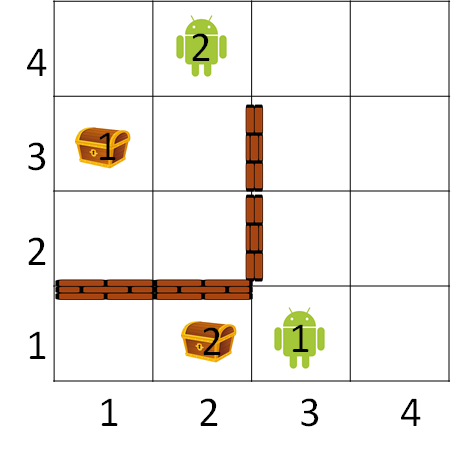
\includegraphics[scale=0.3]{Figures/G.png}
      \caption{$G$}
      \label{fig:G}
    \end{subfigure}
    \begin{subfigure}[b]{0.45\columnwidth}\centering
      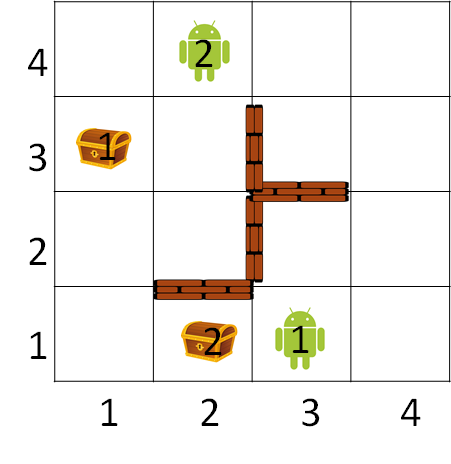
\includegraphics[scale=.3]{Figures/Gs0.png}
      \caption{$G_s$}
      \label{fig:Gs0}
    \end{subfigure}
    \begin{subfigure}[b]{0.45\columnwidth}\centering
      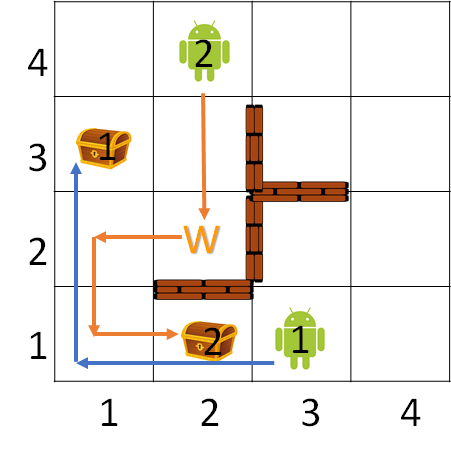
\includegraphics[scale=.3]{Figures/Gs0Plan.png}
      \caption{Snapshot optimal plan}
      \label{fig:PlanGs0}
    \end{subfigure}
    \begin{subfigure}[b]{0.45\columnwidth}\centering
      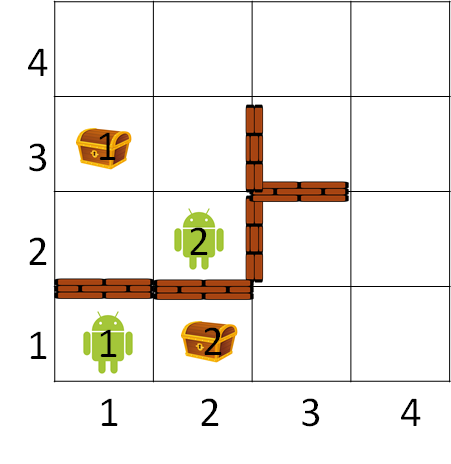
\includegraphics[scale=.3]{Figures/Gs1.png}
      \caption{$G_{s'}$}
      \label{fig:Gs1}
    \end{subfigure}

    \caption{Example MAPF-IM problem}
    \label{fig:ProbelmDefinition}
\end{figure}

\section{Problem Definition}


In MAPF-IM a set of agents must navigate in a graph $G=\langle V, E, \eo, \eb \rangle$, where $E$ is a set of edges, $\eo$ is a set of open edges, while $\eb$ is a set of blocked edges, $E=\eo \cup \eb \land \eo \cap \eb = \emptyset$. The agents are given as input a graph specification $G_s=\langle V, \eko, \ekb, \eao, \eab \rangle$. $G$ denotes the true world graph, while $G_s$ denotes the current knowledge that the agents have about $G$, called the {\em snapshot}. The set of vertices $V$ is identical in $G$ and $G_s$. $\eko$ denotes a set of edges that are known to be open (traversable), i.e, $ e \in \eko \implies e \in \eo$. $\ekb$ denotes a set of edges that are known to be blocked (untraversable), i.e, $e \in \ekb \implies e \in \eb$.
The sets of uncertain edges are denoted by $\eao$ and $\eab$. There may be some edges $e\in \eao \cap \eb$, i.e, an edge the agents assume may be open, but may actually be missing from the graph. Similarly, there may be some edge $e' \in \eab \cap \eo$, that is, an edge the agent assumes is blocked, yet it may actually exists in the underlying graph.

We further assume that the input specification is mostly accurate. That is, $| \eao \cap E_b | \ll |\eao \cap E_o|$ and $| \eab \cap E_o | \ll |\eab \cap E_b|$.
The following properties hold for any snapshot:
$\eko \cap \ekb = \emptyset$, $\eao \cap \eab = \emptyset$, $\eko \cap \eao = \emptyset$, and $\ekb \cap \eab = \emptyset$.
% The following properties hold for any snapshot:
% (1) $\eko \cap \ekb = \emptyset$, (2) $\eao \cap \eab = \emptyset$, (3) $\eko \cap \eao = \emptyset$
% \begin{itemize}
%     \item $\eko \cap \ekb = \emptyset$.
%     \item $\eao \cap \eab = \emptyset$.
%     \item $\eko \cap \eao = \emptyset$.
%     \item $\ekb \cap \eab = \emptyset$
% \end{itemize}
% That is, the agents are certain about an edge or assume the edge is either open or blocked.
Let $O(v, e)$ be an observation relation between vertex and edge. When an agent is at vertex $v$, it observes whether an edge $e$ exists, i.e, $e \in \eo \lor e \in \eb$. Given the current snapshot $G_s$ and the joint action, the agents arrive at the vertices $V_{new}= \langle v_1, \dots, v_k \rangle$ . After each agent observes the open or blocked edges, a new snapshot $G_{s'} = \langle V, \eko', \ekb', \eao', \eab' \rangle $ is obtained such that:
\begin{itemize}
    \item $\eko' = \eko \cup \{e \in \eo \mid \exists v_i \in V_{new} \land \langle v_i, e \rangle \in O(v_i, e)\}$. The set of all edges that were detected from the new positions of the agents.
    \item $\ekb' = \ekb \cup \{e \in \eb \mid \exists v_i \in V_{new} \land \langle v_i, e \rangle \in O(v_i, e)\}$. The set of non existing edges that were detected from the new positions of the agents.
    \item $\eao' = \eao \setminus \{e \mid \exists v_i \in V_{new} \land e \in \eao \cap \ekb' \land \langle v_i, e \rangle \in O(v_i,e)\}$. The set of all edges that the agents assumed to exist but were detected to be missing.
    \item $\eab' = \eab \setminus \{e \mid \exists v_i \in V_{new} \land e \in \eab \cap \eko' \land \langle v_i, e \rangle \in O(v_i,e)\}$. The set of all edges that the agents assumed were missing, but were detected to exist.
\end{itemize}

\commentout{
A solution to MAPF-IM is a \emph{policy} \guy{I do not think that we need this, because we never compute such a policy.}
\begin{equation}
    \pi(G_s, \langle v_1, \dots, v_k\rangle) = \langle a_1 \ldots, a_k \rangle
\end{equation}
specifies the joint action considering the current snapshot and the agent's locations.
}

\commentout{
\guy{Consider the paragraph below as an alternative definition for snapshots:} A {\em snapshot} is a CMAPF specification $G=\langle V, E, \eo, \eb \rangle$ at a particular time during the navigation process.
Given any MAPF-IM problem $G_s=\langle V, \eko, \ekb, \eao, \eab \rangle$, the resulting snapshot is $snap(G_s)=\langle V, \eko \cup \eao, \ekb \cup \eab \rangle$, that is, we assume that all edges that are assumed to be open, are indeed open, and all edges that are assumed to be closed, are indeed closed.
The initial snapshot is based on the input problem specification, and after each observation the snapshot is revised.
}

It is desirable to reach the goal at the minimal amount of steps. However, agents may not know initially which path would yield a lower number of steps, as they have only partial information about open and blocked edges. We hence restrict our attention to {\em snapshot optimality}. Given a snapshot $G_s$, the action that the agents take must be the first action in some minimal cost collision-free plan, assuming that $G_s$ is accurate. That is, assuming that the true graph is $G'=\langle V, \eko \cup \eao \rangle$.
\commentout{$\eko \cup \eao = \eo \land \ekb \cup \eab = \eb$.}

% \nir{optional}

% \nir{It might be preferable to present the 'distributed' algorithm as an improvement: we may benefit from planning snapshot optimal policy only for adjacent agents since the underlying graph is unreliable and generating policies for high number of agents is redundant and runtime-consuming}

% MAPF-IM introduces a new action $sense$
% \begin{equation}
%     sense(v_{c_i}) = \{{v_{c_j} \mid a_i, a_j \in A \land d(v_{c_i}, v_{c_j}) <= R}\}
% \end{equation}
% $v_{c_i}, v_{c_j}$ denotes the current locations of agents $a_i, a_j$ respectively. $d(v_{c_i}, v_{c_j})$ defines the distance within agents can communicate with each other.

% In centralized execution, we presume $R=\infty$, thus all agents can communicate and share their observations. A snapshot is unique and built based on all agent's observations.

% In distributed execution, we assume $R < \infty$, hence agents can communicate within a bounded distance. An agent maintain a \emph{private snapshot} $G_s^i=\langle V, \eko^{i}, \ekb^{i}, \eao^{i}, \eab^{i} \rangle$. Agents share their private snapshots with adjacent neighbors, thus establishing a \emph{group}. A group $g_l$ generates a snapshot $G_s^{g_l}$ considering only its members private snapshots, i.e, $G_s^{g_l}=\langle V, \bigcup_{i=1}^m \eko^{i}, \bigcup_{i=1}^m \ekb^{i}, \bigcap_{i=1}^m \eao^{i}, \bigcap_{i=1}^m \eao^{i} \rangle$. We consider the intersection of uncertain edges since all agents are given the same input graph and broadcast their private snapshot to their neighbors. Therefore, an edge remains uncertain as long as no agent observed it, i.e, $\forall i: e \notin \eko^{i} \land e \notin \ekb^{i}$.

\begin{example}
In Figure~\ref{fig:ProbelmDefinition} the vertices $V$ are the grid cells and the edges $E$ are edges to neighboring cells in the 4 principle directions. For example, $\langle (1,1) , (2,1)\rangle \in E$, and also $\langle (1,1) , (1,2)\rangle \in E$. $\eo$ is the set of open edges, in this case, adjacent cells with no wall in between, and $\eb$ is the set of blocked edges, i.e, adjacent cells with walls in between. For example $\langle (1,1) , (2,1)\rangle \in \eo$ and $\langle (1,1) , (1,2)\rangle \in \eb$ (Figure~\ref{fig:G}).
In the first snapshot (Figure~\ref{fig:Gs0}), $\eao$ is almost identical to the true $\eo$ except for edge $\langle (1,1), (1,2) \rangle \in \eao \setminus \eo$. Similarly, $\eab$ contains all edges in $\eb$, except for the edge $\langle (3,2), (3,3) \rangle \in \eab \setminus \eb$.
The planned policies are shown in Figure~\ref{fig:PlanGs0}. After executing the first joint action, the agents did not observe any new information, hence the snapshot remains the same. Yet, after performing the second joint action, agent $a_1$ observed that $e=\langle (1,1) , (2,1)\rangle$ is blocked, i.e $e \in \eb$. Thus, a new snapshot $G_{s'}$ (Figure~\ref{fig:Gs1}) is obtained where $e \in \ekb' \land e \notin \eao'$. That is, in the new snapshot the agents are certain that $e$ is blocked, therefore any future policy must avoid traverse this edge.
\end{example}




% \section{Problem Definition (Guy)}

% \guy{this definition seems one-sided. }
% In MAPFUN a set of agents must navigate in a graph $G=\langle V, E \rangle$. However, the agents are given as input a graph specification $G_s=\langle V, E_k, E_u \rangle$. $G$ denotes the true world graph, while $G'$ denotes the current knowledge that the agents have about $G$, called the {\em snapshot}.
% The set of vertices $V$ is identical in $G$ and $G_s$. $E_k$ denotes the set of known edges, that is $\forall e \in E_k, e \in E$. $E_u$ denotes the of unknown edges, that is, there may be some edges $e\in E$, $e\notin E_u$, and there may be some edges $e' \in E_u, e' \notin E$.

% \guy{Suggesting below a symmetric definition.}

% In MAPFUN a set of agents must navigate in a graph $G=\langle V, E \rangle$. The agents are given as input a graph specification $G_s=\langle V, E_k,E_{\overline{k}}, E_u,E_{\overline{u}} \rangle$. $G$ denotes the true world graph, while $G'$ denotes the current knowledge that the agents have about $G$, called the {\em snapshot}.
% The set of vertices $V$ is identical in $G$ and $G_s$. $E_k$ denotes the set of known edges, that is $\forall e \in E_k, e \in E$. $E_{\overline{k}}$ denotes the set of edges that are known to be missing, that is $\forall e \in E_{\overline{k}}, e \notin E$.
% $E_u$ and $E_{\overline{u}}$ denote uncertain edges. There may be some edges $e\in E_u$, $e\notin E$, and there may be some edges $e' \in E_{\overline{u}}, e' \in E$. That is, $E_u$ contains edges that the agents believe may exist, but may actually be missing from the graph $G$, while $E_{\overline{u}}$ may contain edges that the agents believe are missing, but may exist in $G$.

% \begin{itemize}
%     \item $E_k \cap E_{\overline{k}} = \emptyset$
%     \item $E_u \cap E_{\overline{u}} = \emptyset$
%     \item $E_u \cap E_k = \emptyset$
%     \item $E_{\overline{u}} \cap E_{\overline{k}} = \emptyset$
% \end{itemize}


% \plan{Implicit observations - observation relation $O(v,e)$ between vertex and edge. When reaching a vertex you observe all edges that satisfy the relation. After observing you get a new snapshot $G_{s'}$ where some edges move from $E_u$ to $E_k$.}

% $O(v, e)$ -- if an agent is at $v$ it observes whether $\langle e \rangle \in E$.

% \plan{Alternative definition for $O$}

% Let $O$ be an observation function. That is, $O(v)$ is the set of ???


% \plan{Explain how, given $O$ we get $G_{s'}$}
% Given the current snapshot $G_s$, and a joint action, the agents arrive at vertices $V_c=\langle v_1, \ldots, v_n \rangle$. The new snapshot $G_{s'}=\langle V,E'_k,E'_{\overline{k}}, E'_u,E'_{\overline{u}} \rangle $ contains:
% \begin{itemize}
%     \item $E'_k = E_k \cup \{ \langle v_j,v_l \rangle | \exists v_i \in V_c, O(v_i,\langle v_j,v_l \rangle),  \langle v_j,v_l \rangle \in E\}$ -- the set of all edges that were detected from the new positions of the agents.
%     \item $E'_{\overline{k}} = E_{\overline{k}} \cup \{ \langle v_j,v_l \rangle | \exists v_i \in V_c, O(v_i,\langle v_j,v_l \rangle),  \langle v_j,v_l \rangle \notin E\}$ -- the set of all non existing edges that were detected from the new positions of the agents.
%     \item $E'_u = E_u \setminus \{ \langle v_j,v_l \rangle \in E_u | \exists v_i \in V_c, O(v_i,\langle v_j,v_l \rangle),  \langle v_j,v_l \rangle \notin E\}$ -- the set of all edges that the agents assumed to exist but were detected to be missing.
%     \item $E'_{\overline{u}} = E_{\overline{u}} \cup \{ \langle v_j,v_l \rangle \in E_{\overline{u}} | \exists v_i \in V_c, O(v_i,\langle v_j,v_l \rangle),  \langle v_j,v_l \rangle \in E\}$ -- the set of all edges that the agents assumed were missing, but were detected to exist.
% \end{itemize}


% \plan{Solution - policy $\pi(G_s,\langle v_1,...,v_n \rangle)$ specifies which action each agent should take given the current snapshot and all agent locations.}

% \plan{Optimality criterion - similar to contingent planning, no good way to compare policies (plan trees), and we hence assume snapshot optimality - optimal if the current knowledge is accurate. Discussion - this criterion does not prefer moving through known edges, this criterion does not take value of information into account.}


% \section{Problem Definition (Nir)}
% \plan{A maps is given}

% \plan{There is uncertainty - some open cells may be blocked, some blocked cells may be open}
% \guy{Uncertain maps does not sound good. I suggest, inaccurate maps.}

% We now describe an extension to CMAPF that we call \emph{multi-agent path finding under uncertain maps (MAPFUM)}

% \guy{I suggest the following formal definition:}
% In MAPFUN a set of agents must navigate in a graph $G=\langle V, E \rangle$. However, the agents are given as input a graph specification $G_s=\langle V, E_k, E_u \rangle$. $G$ denotes the true world graph, while $G'$ denotes the current knowledge that the agents have about $G$, called the {\em snapshot}.
% The set of vertices $V$ is identical in $G$ and $G_s$. $E_k$ denotes the set of known edges, that is $\forall e \in E_k, e \in E$. $E_u$ denotes the of unknown edges, that is, there may be some edges $e\in E$, $e\notin E_u$, and there may be some edges $e' \in E_u, e' \notin E$.


% \guy{I think that we now need a definition of sensing. I suggest to define a distance metric $d(v,v')$, and say that if $d(v,v')<c$ then an agent in $v$ can sense all outgoing edges from $v'$. Alternatively, maybe we just want a relation and not a distance metric, because I do not think that line of sight respects the triangle inequality.}

% \guy{your definition below. I am unsure whether we need the term "uncertain edges" - it seems like you know which edges are uncertain. If you do need this, then you can use $UE= (E \cup E') \setminus (E \cap E')$}
% In MAPFUM, a subset of edges might be added or removed. We refer to these subset as \emph{uncertain edges (UEs)}. Initially, the agents are not aware whether an edge is traversable. Thus, the UEs refers to as the \emph{online} part of the problem, whereas the map and set of agents refers to as the \emph{offline} part of the problem. \guy{This is not what online and offline usually refer to. Typically, offline is solving before acting, and online means interleaving solving and acting. Better not to overload terms.}

% \guy{The paragraph below discusses the solution, which does not belong in this section. The solution would be in the next section.}
% An online MAPFUM starts by solving an offline MAPF problem. While the agents following their destined trajectories, they \emph{observe} which edges are traversable. An \emph{observation} is a triplet, $\langle e, s, t\rangle$, where $e$ is an uncertain edge, $s$ is the edge \emph{status}, $t$ is the timestep. Upon perceiving a new observation, a replanning is required, take into account the new knowledge about the map. Formally, MAPFUM is a quintuplets $\langle G, A, UE, F, O \rangle$, where G, A are defined as in CMAPF. $UE \subset E$ is the set of uncertain edges.
% \plan{Sensing obstacles - within given range - we see all blocked and unblocked cells}

% \guy{I am not sure that we need the term edge configuration, certainly not for the algorithm. If anything, then we would need it for proofs (??). I do not think that it should be a part of the problem definition.}
% An \emph{edge configuration} $$F: (UE \times \mathbb{N}^+) \rightarrow  \{open, closed, unkown\}$$ is a mapping between a UE at a specific timestep to its state. We included here an artificial state \emph{unknown}, to enable representing incomplete knowledge of an edge status. This state is used to model an edge configuration in which the problem-solvers does not know yet the state of an edge $e \in UE$.

% \guy{Do not use \$\$. Instead use begin\{equation\} end\{equation\}.}
% An \emph{observation function} over any $v \in V$
% $$O(v) = \{\langle e, F(e, t), t \rangle \mid e=(v_{i}, v_{j}) \in U, d(v, v_{i}) \le R\}$$
% \guy{I think that the definition should include two vertices. as I said above.}
% defines the range within an agent can observe an uncertain edge. That is, an agent at vertex $v_{s}$ can reveal uncertain edges status at timestep $t$ within proximity factor $R$ from the edge source $v_{i}$.

% The set of actions in MAPFUM contains move and wait actions, as well as the observe action, which precedes both of them \guy{we need to discuss this - do we want implicit or explicit observations. I think that implicit observations make more sense here. Your definition seems implicit, but then there is not need for an "observe" action - it is enough to say that the agent observes all edges within range.}. That is, an action starts with observing adjacent edges. If new observation is received, new paths are generated, considering the current knowledge about the map. Otherwise, the previously planned trajectories are followed.

% \guy{Your paragraphs jump from one topic to the other. You talked about configurations two paragraphs ago.}
% We say that \emph{edge configuration} is \emph{consistent} if its state is permanent throughout the execution and is either open or closed, i.e,
% $$\forall e \in UE, \forall t_{1}, t_{2} \in \mathbb{N}^+: F(e, t_{1}) = F(e, t_{2})$$
% In our setting, we assume consistent edge configuration to benefit from sharing observations among agents. \guy{this is not what consistency means. I think that you mean fixed or stationary, as opposed to dynamic.}
% \plan{Goal - snapshot optimality}

% \guy{We need to discuss the solution as well. The solution is obviously a tree, but this tree, assuming that we do not know which edges are inaccurate, is too big. There will never be an offline tree computation algorithm. Need to discuss this.}
% A solution to MAPFUM is a sequence of CMAPF plans,
% $$\Lambda = \langle \Pi^{t_{0}}, \Pi^{t_{1}}, \ldots, \Pi^{t_{m}}, \Pi^{t_{\infty}} \rangle$$
% $\Pi^{t_{i}}$ is a \emph{partial plan} which were executed until a new observation is perceived at timestep $t_{i}$, necessitates replanning and thus generating the $\Pi^{t_{i+1}}$ plan.
% $\Pi^{t_{0}}$ is the plan for the offline input. $\Pi^{1 \le t_{i} \le m}$ is generated considering the observations that were gathered until timestep $ t_{i}$.
% $\Pi^{t_{\infty}}$ represents the last generated plan afterwards all agents attained their goals.




% \subsubsection*{Objective Function}
% \guy{do not use * after section or subsection. Also need to respect the hierarachy - section, subsection, subsubsection.}

% \guy{Not sure that the term "objective function" is accurate. We do not have an optimization problem here. I think that we need to tak a bit about what would amount to be an optimal solution. Not sure that I have a good answer.}

% We generalize the notion of SOC to an online setting:
% $$Online-SOC(\Lambda)=\Sigma_{i=0}^{\infty} SOC(\Pi^{t_{i}})$$
% It is the sum over the partial plans until all agents reached their goals.
% Porting the definition of \emph{snapshot optimal} from Svancara et al. (2019), we say that partial plan $\Pi^{t_{i}}$ is snapshot optimal, if it is minimal in terms of SOC, considering the knowledge obtained until timestep $t_{i}$.
% We denote by $OPT^{t_{i}}$ a snapshot optimal partial plan.
% A MAPFUM solution is optimal if any of its partial plans is snapshot optimal, i.e,
% $$\forall t_{i}: SOC(\Pi^{t_{i}})=SOC(OPT^{t_{i}})$$
% Hence, a MAPFUM solution $\Lambda$ is optimal with respect to Online-SOC iff
% $$Online-SOC(\Lambda)=\Sigma_{i=0}^{\infty}SOC(\Pi^{t_{i}})=\Sigma_{i=0}^{\infty} SOC(OPT^{t_{i}})$$


%%%%%%%%%%%%%%%%%%%%%%%%%%%%%%%%%%%%%%%%%%%%%%%%%%%%%%%%%%%%%


\begin{algorithm}[t]
\caption{Online Replanning}
    \label{alg:generic}
\footnotesize
\SetKwBlock{Main}{Main}{end}
\SetKwInOut{Input}{Input:}
\SetKwInOut{Output}{Output:}
\Input{Snapshot $G_s=\langle V, \eko, \ekb, \eao, \eab \rangle$, Observation relation $O$, Set of agents $A$}
    $t \leftarrow 0$\\
    $\pi \leftarrow Init(G_s, \emptyset, G, A, t)$ \\
    \While{not all agents reached their goals}{
        $G'_s \leftarrow UpdateSnapshot(G_s, A, O)$\\
        \If{$G_s \neq G'_s$}{
            $\pi \leftarrow Replan(G'_s, \pi, G, A, t)$\\
            $G_s \leftarrow G'_s$
        }
        $Execute(\pi[t])$ \\
        $t \leftarrow t + 1$
    }
    \Return{$\pi$}
\end{algorithm}


\section{Online Planning Framework}

We now describe our online replanning approach for solving MAPF-IM problems. The agents act based on their current knowledge of the world, assuming that the given snapshot is accurate. %graph definition is accurate.
Whenever new information becomes available to one agent, it communicates the information to all agents. Then, the agents may replan given the new information.

We use an online replanning approach because an offline planner, that plans for all contingencies ahead before acting, must, in our case, create huge plan trees, branching at every step, given the multitude of possible observations. As we assume that the graph specification is mostly accurate, planning for extremely unlikely contingencies is wasteful.

Below, we describe our online algorithms. We begin with a generic replanning algorithm, emphasizing the main components of all replanning methods. Algorithm~\ref{alg:generic} shows this generic algorithm. The algorithm begins with initializing the multi-agent plan (line 3), and then the agents start acting.

At each step the agent update the current snapshot given the observation function $O$, that is, all edges that are observable from the current positions of the agents are observed, and the agents communicate their observations to form a centralized new snapshot. If the snapshot is identical to the previous one, then the existing plan is still valid, and the agents can continue to act.

If the new snapshot is different (line 6), because an edge that was deemed to be open is blocked, or because an edge believed to be blocked is actually open, then a replanning is triggered (line 7).
The agents execute the plans (line 8) until all agents reach their goals (line 4).

We now describe a set of possible implementations for {\em Init} and {\em Replan}. First, we suggest a naive approach which we call {\em AlwaysReplan}. This method initializes the plan using any CMAPF method, and replans from scratch following every observation, again using a CMAPF method. Given an optimal CMAPF solver, this ensures snapshot optimality, as the agents recompute their plans given the current snapshot.


However, this approach can be  wasteful. First, not all observations are relevant to the agents. We hence later suggest a mechanism to identify whether a new observation can be relevant to an agent. Second, we can leverage information from previous CMAPF computations to reduce the replanning effort. We describe these improvements in Section~\ref{scn:IDCBS}.

A CMAPF solver resolves all collisions before starting to act. However, in MAPF-IM, we expect that new information would cause the agents to alter their paths. Thus, possible collisions that would occur far from the current positions of the agents may no longer be relevant, given the revised paths. Using this intuition we can suggest a second approach, that resolves only collisions that occur within at most $r$ timesteps from the current position of the agents. We describe this approach in Section~\ref{scn:local}.


An interesting question arises with respect to deadends. Our approach assumes no deadends, that is, there is a CMAPF solution in the true graph $\langle V, E_o \rangle$. However, our algorithms currently employ an even stronger assumption, that given the initial snapshot $G_s=\langle \eko, \ekb, \eao, \eab \rangle$, there exists a solution in the set of edges $\eko \cup (E_o \cap \eao)$. That is, the blocked edges in $\eao$ do not cause a deadend.

From the algorithmic point of view, this assumption is not needed.
We can modify our algorithms above such that if there is no CMAPF solution in $\langle V, \eko \cup \eao \rangle$, then we look for a CMAPF solution in $\langle V, \eko \cup \eao \cup \eab \rangle $, that is, we assume that all edges that were believed to be blocked are in fact open. If there is a solution in the true graph, then there is also a solution in this graph as well. Another question that arises then is the problem of smart exploration strategies to identify the open edges in $\eab$.

One could take this approach to begin with, but as the number of open edges in $\eab$ is expected to be very small, this approach would not be efficient, exploring multiple blocked edges. In addition, without the assumption above, the definition of snapshot optimality is not well defined. We hence make the above assumption, and leave further discussions of deadends to future research.




\begin{algorithm}[t]
\caption{Replan, ID + PP}
    \label{alg:replanidpp}
\footnotesize
\SetKwBlock{IDPPReplan}{Replan($G_s, \pi, A, t$)}{end}
\SetKwInOut{Input}{Input:}
\SetKwInOut{Output}{Output:}
\IDPPReplan{
\Input{new snapshot $G_s$, ongoing policy $\pi$,  set of agents $A$, current timestep $t$}
    $G\leftarrow \langle V, \eko \cup \eao \rangle$\\

    $A_r \leftarrow \{a_i \in A : \mbox{affected}(\pi_i, G_s)\}$\\
    $A_{\overline{r}} \leftarrow A \setminus A_r$\\
    $\pi' \leftarrow PP(G, \pi, A_r, A_{\overline{r}})$\\
    \If{$\pi'=\emptyset$}{
        $\pi' \leftarrow PP(G, A)$
    }
    Revise $\pi$ using $\pi'$\\
    \Return{$\pi$}
    }
\end{algorithm}

\commentout{
    \begin{algorithm}[t]
    \caption{Replan, ID + PP \nir{new}}
        \label{alg:replanidppnir}
    \footnotesize
    \SetKwBlock{IDPPReplan}{Replan($G_s, \pi, A, t$)}{end}
    \SetKwInOut{Input}{Input:}
    \SetKwInOut{Output}{Output:}
    \IDPPReplan{
    \Input{new snapshot $G_s$, ongoing policy $\pi$,  set of agents $A$, current timestep $t$}
        $G\leftarrow \langle V, \eko \cup \eao \rangle$\\
        $A_r \leftarrow \{a_i \in A : \mbox{affected}(\pi_i, G_s)\}$\\
        $\pi' \leftarrow \emptyset$\\
        \While{$ \pi' = \emptyset \wedge |A_r| < |A|$}{
            $A_{\overline{r}} \leftarrow A \setminus A_r$\\
            $\pi' \leftarrow PP(G, \pi, A_r, A_{\overline{r}})$\\
            \If{$\pi'=\emptyset$}{
                $\hat{p} \leftarrow \min_{i=1}^{|A_r|}\mbox{P}(i)$\\
                $A_r \leftarrow A_r \cup \{a_j \in A_{\overline{r}} \mid \mbox{P}(j)>\hat{p} \}$ \\\tcp{add all unaffected agents with priority higher than the lowest priority affected agent}
            }
        }
        \If{$\pi' = \emptyset$}{
            $\pi' \leftarrow PP(G, A)$
        }
        Revise $\pi$ using $\pi'$\\
        \Return{$\pi$}
        }
    \end{algorithm}
}


\begin{algorithm}[t]
\caption{Replan, ID + CBS}
    \label{alg:replanidcbs}
\footnotesize
\SetKwBlock{IDCBSReplan}{Replan($G_s, \pi, A, t$)}{end}
\SetKwInOut{Input}{Input:}
\SetKwInOut{Output}{Output:}
\IDCBSReplan{
\Input{new snapshot $G_s$, ongoing policy $\pi$, set of agents $A$, current timestep $t$}
    $G\leftarrow \langle V, \eko \cup \eao \rangle$\\
    $C \leftarrow \{ c \in C_\pi : t(c)>t\}$\\
    $groups \leftarrow Partition(C)$\\
    \ForEach{$g \in groups$}{
        \If{$\exists a_i \in g , \mbox{affected}(\pi_i,G_s)$}{
            $C \leftarrow C \setminus C_g$ \\
            $\pi_g, C_g \leftarrow CBS(G, g)$\\
            Revise $\pi$ using $\pi_g$\\
            $C \leftarrow C \cup C_g$
        }
    }
    \While{$\exists g_i, g_j \in groups$ with colliding paths}{
        $g \leftarrow g_i \cup g_j$\\
        $groups \leftarrow (groups \cup g) \setminus g_i,g_j$\\
        $C \leftarrow C \setminus C_g$\\
        $\pi_g, C_g \leftarrow CBS(G, g)$\\
        Revise $\pi$ using $\pi_g$\\
        $C \leftarrow C \cup C_g$\\
    }
    $C_\pi \leftarrow C$\\
    \Return{$\pi$}
    }
\end{algorithm}



\subsection{Reducing Replanning Computations}
\label{scn:IDCBS}

Replanning using a CMPAF planner for all agents following every new observation might be costly.
It is desirable to reuse the computations from previous replanning episodes to expedite the next replanning episodes.

First, we would want to limit the replanning only to agents that are affected by the new information, as often, some of the agents policies might be unaffected. The effect of an edge that was considered open (in $\eao$) but is blocked (in $\ekb$) can be tracked by identifying agents that intended to move through that edge. Identifying whihc agents are affected by an edge that was thought to be blocked (in $\eab$) but is open (in $\eko$) is more challenging. We assume here that if the new open edge allows an agent to shorten its current path to the goal, then it is relevant for it.
We now suggest two methods that use the above intuition to replan only to agents that are affected by new knowledge about edges. Each method is based on using a particular CMAPF solver, either prioritized planning (PP) or CBS.
%\roni{Maybe instead say that one method is geared towards finding low-cost solutions while the other is geared towards optimizing runtime.}\guy{feel free to edit as you see fit}


Algorithm~\ref{alg:replanidpp} uses a PP approach for the replanning phase in Algorithm~\ref{alg:generic} (line 7). We use a prioritization scheme where agents whose paths are not affected by the new knowledge are considered to be of higher priority. Hence, the algorithm attempts to replan only for the affected agents, denoted $A_r$ (line 3). Thus, when we call PP (line 5), the paths of agents in the complement $A_{\overline{r}}$ are considered fixed, and agents in $A_r$ plan to avoid them. Of course, this may fail because, e.g., and agent in $A_{\overline{r}}$ might be at its goal position, and thus will not move, and it blocks the path of another agent. Hence, if running PP only for agents in $A_r$ fails (line 6), we replan for all agents (line 7). We revise the plan $\pi$, replacing the plans that changed starting from time $t$ (line 8).

Our second approach is based on CBS, attempting again to replan only for some of the agents. As CBS resolved conflicts, it constrains several agents. Hence, if one agent must change its path, this may cause other agents to alter their paths as well.
We suggest here to identify groups of agents that might collide and plan for each group independent of other groups, similar to the ID approach. To identify these groups, we use the resolved conflicts $C_\pi$ computed by the CBS algorithm when computing a policy $\pi$ in a previous iteration. Every two agents for which CBS previously identified a conflict after the current time, are at risk of colliding, and are therefore added to the same group.
After replanning for each group independently, we check whether the new plans cause agents from different groups to collide, and if so, using an ID approach, unite the groups and replan.

Algorithm~\ref{alg:replanidcbs} describes this replanning process. First, we identify a set of conflicts $C$ that were computed for the previous policy $\pi$, and are still relevant, i.e., occur after the current step $t$ (line 3). We partition the agents into disjoint groups (line 4) given $C$. We consider pairs of agents $a_i,a_j$ such that there exists a conflict in the set $C$. Each such pair $a_i,a_j$ must be in the same group.

Given the set $groups$, we call CBS on each group $g$ that is affected by the new knowledge independently (lines 5-10). A group $g$ is affected if there is an agent $a \in g$ that is affected. An agent is affected by a new blocked edge $e_1$ if its current path passes through $e_1$. An agent is affected by a new open edge $e_2$ if the shortest path from its current position to the goal, that passes through $e_2$, is shorter than its current path to the goal, that is, if its current path can be shortened by passing through $e_2$. We use another insight to avoid multiple calls to $A^*$. Given an admissible heuristic $h$, we compute the sum of heuristic costs from the current position of the agent to $e_2$, and from $e_2$ to its goal. Only if that cost is lower than its current path to the goal, we replan. In addition, we replace the conflicts relevant for $g$ with the new conflicts generated during replanning (lines 7,10).

After planning for each group $g$ independently, we check whether new plans for agents from different groups now collide (line 11). As long as such two groups $g_i,g_j$ exist,  we join them into a new group $g$ (lines 12-13), we remove the conflicts associated with the joint group $g$  (line 14), and replan for $g$ (line 15).
We then check again whether a new collision exists with another group.

\commentout{
We now describe an approach that leverages information gathered from the previous

Obviously, an agent $a_i$ is \emph{affected} only if one of following holds:
\begin{itemize}
    \item New open edge is observed, i.e, $\eko' \setminus \eko \ne \emptyset$. Re-routing the agent might decrease the policy cost, hence necessary to guarantee snapshot optimality.
    \item New blocked edge is observed and $a_i$ plans to cross it, i.e, $\exists t: Execute(\pi_i[t]) \cap \ekb' \neq \emptyset$. Replanning is obligatory to guarantee soundness.
\end{itemize}
Thus, we can enhance the RA performance by replanning only for affected agents. However, had we re-routed an agent, we might might free up locations that were prohibited to occupy by other agents, because of a possible collision, thus perhaps shorten their pathways\nir{quote roni?}. Therefore, we must replan for an affected agents, as well as the agents that he will collide with. That it, we only consider conflicts that shall occur in the future if a pair of agents will blindly follow their shortest path.

CMAPF planning is exponential in the number of agents. Therefore, we would rather partition the agents into disjoint groups such that the optimal path computed for each group do no interfere \nir{quote ID?}. We can establish such a partition by traversing along the CBS goal branch and merging agents that will collide without imposing a constraint. That is, we merge agents that according to their shortest path will collide in the future, i.e, at timestep later than the current step. Notice that merging agents that would had collide is redundant since they are independent of each other from the current timestep.

We conclude that a replanning is necessary only for a group that contains an affected agent, we refer to such a group as \emph{affected group}. Based on this conclusion, we developed the \emph{Independence Detection over Conflict Based Search (ID+CBS)} algorithm. The major distinction between ID+CBS and RA is that ID+CBS exploits previous knowledge from prior planning phase. In ID+CBS, once a new policy is required, we partition the agents into disjoint groups based on future collision that were detected by the CBS while generating the ongoing policy.
Thereafter, we update the current policy only for affected groups. Finally, we apply CBS search where the root node is initialized with the updated policy to resolve possible further conflicts between the groups. That is, we commence the CBS search with a well-informed starting point instead of shortest path for each agent.\nir{We can apply ID over the disjoint group, planning for each group with CBS to maintain collision. However, in the experiment it  performs same as running CBS starting with the modified policy. }

Algorithm ~\ref{alg:ID+CBS} lists the pseudo code for ID+CBS. Similar to RA, we outset with generating a policy for the input snapshot. However, we run CBS for this sake to maintain the conflicts that were resolved during the search (lines 2-3). The $\emptyset$ specifies that the CBS search starts with an uninformed starting point, i.e, the root node is initialized with shortest path for each agent while ignoring all other agents. Next, the agents move to execute their designed policies, while observing new information (line 4-5). Once the snapshot is changed, we partition the agents into disjoint groups based on future conflicts (line 8). Then, we update the ongoing policy for the affected groups (lines 10-11). Eventually, we start a CBS with the modified policy (line 12).
}

\begin{algorithm}[t]
\caption{Local Conflict Resolution}
    \label{alg:local}
\footnotesize
\SetKwBlock{Main}{Main}{end}
\SetKwInOut{Input}{Input:}
\SetKwInOut{Output}{Output:}
\Input{Snapshot $G_s=\langle V, \eko, \ekb, \eao, \eab \rangle$, Observation relation $O$, Set of agents $A$, Proximity radius $r$}
    $t \leftarrow 0$\\
    $\pi \leftarrow Init(G_s, \emptyset, G, A, r, t)$ \\
    \While{not all agents reached their goals}{
        $G'_s \leftarrow UpdateSnapshot(G_s, A, O)$\\
        \If{$G_s \neq G'_s$}{
            $\pi \leftarrow Replan(G'_s, \pi, G, A, t, r)$\\
            $G_s \leftarrow G'_s$
        }
        \If{$\exists a_i,a_j : collide(\pi_i, \pi_j, t, r)$}{
            $\pi \leftarrow ResolveCollisions(\pi,A,G_s,t,r)$
        }
        $Execute(\pi[t])$ \\
        $t \leftarrow t + 1$
    }
\end{algorithm}



\subsection{Local Conflict Resolution}
\label{scn:local}
Limiting the horizon in which conflicts are considered during planning has been shown to be effective in different MAPF contexts~\cite{silver2005cooperative,li2021lifelong}. This technique is expected to work well for MAPF-IM as well, since agents are likely to change their paths due to new information, and thus resolving conflicts that far in the future is wasteful. Specifically, when replanning we only consider conflicts that are at most $r$ steps from the current state, where $r$ is a parameter. To ensure a safe execution, we monitor the agents' location during execution, and call for replanning if a conflict is about to occur within the next $r$ steps.
We refer to this approach as \emph{Local Conflict Resolution}. The pseudo-code for this approach is given in Algorithm~\ref{alg:local}. %provide a high-level pseudo-code to describe
% If we limit our attention only to conflicts that would occur in the near future, we can reduce this wasted effort.
% Inspired by the success of this approach
% Consider conflicts
% We now describe a method that resolves conflicts only for agents that will collide within at most $r$ steps, where $r$ is a proximity parameter. The intuition behind this approach is that agents are likely to change their paths due to new information. Thus, conflicts that were detected may no longer apply after path changes, and resolving these conflicts is wasteful. If we limit our attention only to conflicts that would occur in the near future, we can reduce this wasted effort.

%%%%%%%%%%%%%%% COMMENNNNNTED OUT
% Algorithm~\ref{alg:local} describes this approach. The algorithm has 3 main subroutines : initialization (line 3), where an initial plan is computed, replanning after new information has arrived (line 7), and collision resolution (line 10). We need to check for proximate collisions (line 9) and resolve them, because the computed plans ignore future collisions. Again, as with the approach that resolves all conflicts (Algorithm~\ref{alg:generic}), there can be various implementations for its methods.

% It is possible to use a CMAPF solver, such as CBS or PP (with or without ID), for all 3 subroutines. All these algorithms can be adapted such that they resolve only collisions that occur within at most $r$ steps, ignoring farther collisions~\cite{li2021lifelong}.

% We now explain in detail an approach that can be faster. Instead of using a CMAPF planner, we suggest, both for the initial plan (line 6), as well as for replanning (line 7), to use a single agent planner, such as a best first search or $A^*$. This means that the plan is likely to contain many collisions, that we will handle later on. For replanning, we also limit the replanning to agents that are affected by the new information, as explained in Section~\ref{scn:IDCBS}.

% Before executing the next action, the agents look for collisions. If there are two agents $a_i,a_j$ whose paths $\pi_i,\pi_j$ collide in at most $r$ steps (denoted $collide(\pi_i,\pi_j,r)$), then we must resolve this conflict. We can use here, again, and CMAPF planner, but we suggest here to use the collision resolution method similar to Algorithm~\ref{alg:replanidcbs}. We first partition the agents to groups such that different groups do not collide, and replan using a CMAPF solver for each group independently. If there exist two groups whose new plans collide within the next $r$ steps, we unite them and replan. This is repeated until no agents collide within the next $r$ steps. During this conflict resolution phase we resolve all conflicts in a group, to avoid deadlocks or livelocks, ensuring termination. Similar adaptations can be made to Algorithm~\ref{alg:replanidpp}.\roni{Not clear if this is implemented or just an idea}
%%%%%%%%%%%%%%%%%%%%%%%%%END COMMENTED OUT
\subsection{Theoretical Results}

We say that an observation relation $O$ is \emph{truthful} if for every vertex $v$ and pair of vertices $(u,w)$ it holds that $(v,(u,w))\in O$ if and only if $v=u$ and $(v,w)$ is an edge in the true graph.
\begin{theorem}
Given a truthful observation function,
the Online Replanning framework is (1) sound, i.e., the plan it executes is guaranteed to avoid conflicts and obstacles, if the CMAPF solver is sound; and (2) complete, i.e., if a solution exists then it will eventually be found, if the CMAPF solver is complete.
\end{theorem}
\noindent A proof is given in the supplementary material.


By definition, Online Replanning is snapshot optimal when using \emph{AlwaysReplan} and an optimal CMAPF algorithm such as CBS.
Next, we prove that ID+CBS preserves this property.
\begin{theorem}
   Online Replanning where Replan=ID+CBS is sound and snapshot optimal.
\end{theorem}

\begin{proof}
To prove this theorem, we show that ID+CBS is sound and snapshot optimal when it is given a snapshot optimal policy $\pi$.
    Let $a_1, a_2\in A$ and $\pi_1, \pi_2 \in \pi$ be a pair of agents and their corresponding policies.
    Suppose that $a_1, a_2$ were detected to collide, i.e, $\exists t': \pi_1[t'] = \pi_2[t']$.
    If $t'<t$ it follows that there are no collisions between $\pi_1, \pi_2$ from the current timestep. Therefore, the agents do not affect each other; If one of them frees-up location, it will not affect the other, as it already follows its shortest path. Yet, this is not the case when $t' > t$, since one of the agents was constrained to occupy some vertex that perhaps coerced him to deviate from his shortest path.

    It suffices to show that a group with no affected agent may follow its members' current policies. Let $g$ be such a group, i.e., no affected agent belongs to $g$. By negation, we assume that the ongoing policy for $g$, denoted by $\pi_g$, is either unsound or sub-snapshot-optimal. If $\pi_g$ is unsound, it implies that exists an agent $\hat{a} \in g$ whose planned path traverses a blocked edge. Hence, by definition, $a$ is affected. In contradiction to the initial assumption. If $\pi_g$ is not a snapshot-optimal policy with respect to $g$, it follows that exists a policy $\hat{\pi}$ such that $SOC(\hat{\pi})<SOC(\pi)$. Thus, at least one agent $a \in g$ may shorten his current designated path. Therefore, by definition, $a$ is affected. Contradiction.
\end{proof}


\begin{theorem}
   Given a truthful observation relation $O$ and a proximity parameter $r\ge1$ then Local Conflict Resolution is sound when using a sound CMAPF solver and complete when using a complete SMAPF solver.
\end{theorem}
\noindent A proof is given in the supplementary material.








% \begin{corollary}
% \noindent
%    Online Replanning where Replan=ID+CBS is sound and snapshot optimal.
% \end{corollary}

% \nir{although we can merge those theorems , I think its more clear this way}\roni{I think we will have space constraints, but let's see. }

% \begin{theorem}
%    Given a sound CMAPF solver, a truthful observation relation $O$, and a proximity parameter $r\ge1$ then Local Conflict Resolution is sound.
% \end{theorem}

% \begin{proof}
% \noindent
%     Similar to Online Replanning, on any planning phase merely valid actions are considered. However, conflict resolution is deferred until it detected to occur within at most $r$ steps.
%     Once such a conflict is detected, the ongoing policy is modified by a sound CMAPF planner to resolve it. As $r\ge1$ it follows that the modified ongoing policy is collision-free.
%     % \roni{This is Ok. You can remove this proof and just write ``easy to see'' if we have an issue with space}
% \end{proof}

% \begin{theorem}
%     Given a complete CMAPF solver, an undirected true graph and a proximity parameter $r\ge1$, Local Conflict Resolution is complete.
% \end{theorem}

% \begin{proof}
% \noindent
%     Local Conflict Resoultion behaves similarly to Online Replanning, excluding conflicts resolution. Thus, it suffice to show that deferring collision resolution does not breach completeness. Let $\pi_1, \pi_2 \in \pi$ be a pair of colliding policies and $c$ be the earliest conflict between those policies, such that $\mbox{t}(c) \le r$. Suppose that $ReolveConflicts$ failed. It implies that there are no collision-free policies for the group contains $a_1, a_2$. In contradiction to the true graph property.
% \end{proof}
% % \roni{You can probably merge the two theorems to save space if needed. This proof is Ok, but note that you need here Guy's trick of what to do if your solver says ``no solution''}

\section{Empirical Evaluation}


\begin{figure}[t]
        \centering
    \begin{subfigure}[b]{0.32\columnwidth}\centering
      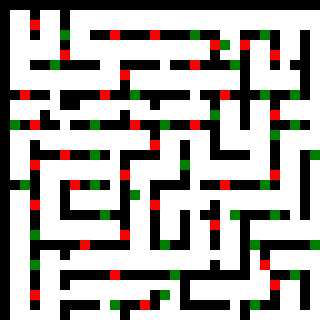
\includegraphics[scale=0.3]{Figures/maze-32-32-2.map.png}
      \caption{Maze}
    \end{subfigure}
    \begin{subfigure}[b]{0.32\columnwidth}\centering
      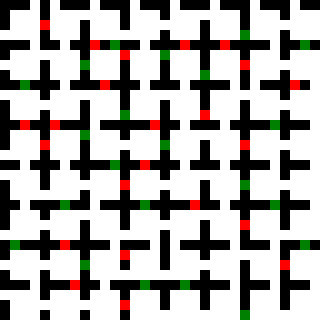
\includegraphics[scale=.3]{Figures/room-32-32-4.map.png}
      \caption{Rooms}
    \end{subfigure}
    % \begin{subfigure}[b]{0.45\columnwidth}\centering
    %   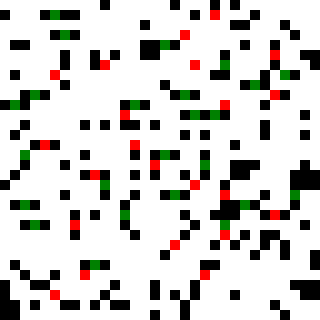
\includegraphics[scale=.3]{Figures/random-32-32-20.map.png}
    %   \caption{Random}
    %   \label{fig:PlanGs0}
    % \end{subfigure}
    \begin{subfigure}[b]{0.32\columnwidth}\centering
      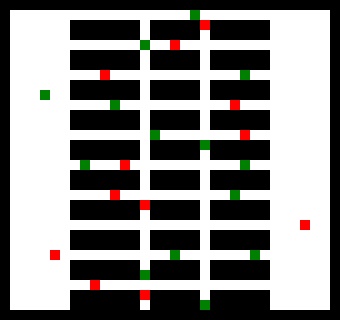
\includegraphics[scale=.3]{Figures/warehouse-32-32.map.png}
      \caption{Warehouse}
    \end{subfigure}
    \caption{Illustrations of the domain types used in our experiments. Green cells denote $\eao$ and red cells denote $\eab$.}
    \label{fig:grids}
\end{figure}

% \plan{Scaling up - given number of agents (on large maps), possible obstacles (on medium sized maps 64), grid size (for rooms and open), different maps (large maps from repository)}
\commentout{
\begin{figure*}[tbhp]
    % \begin{subfigure}[b]{0.9\columnwidth}\centering
    %   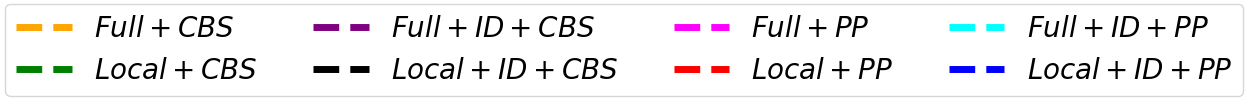
\includegraphics[width=\columnwidth]{Figures/legends-cactus.png}
    %   \caption{Legend}
    %   \label{fig:mazelegends}
    % \end{subfigure}\\
    \centering
    \begin{subfigure}[b]{0.69\columnwidth}\centering
      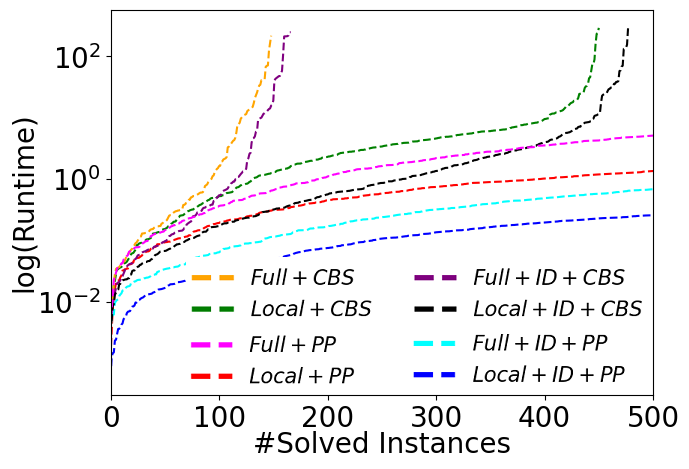
\includegraphics[width=\columnwidth]
      {Figures/maze/mixed_small_figures/Cactus-and-legend.png}
      % {Figures/maze/mixed_small_figures/Cactus.png}
      % \includegraphics[scale=.2]{Figures/maze/mixed_small_figures/DeltaSOC(UEs).png}
      % \caption{Maze grids results.}
      % \label{fig:rt-soc-maze}
    \end{subfigure}
    \begin{subfigure}[b]{0.69\columnwidth}\centering
      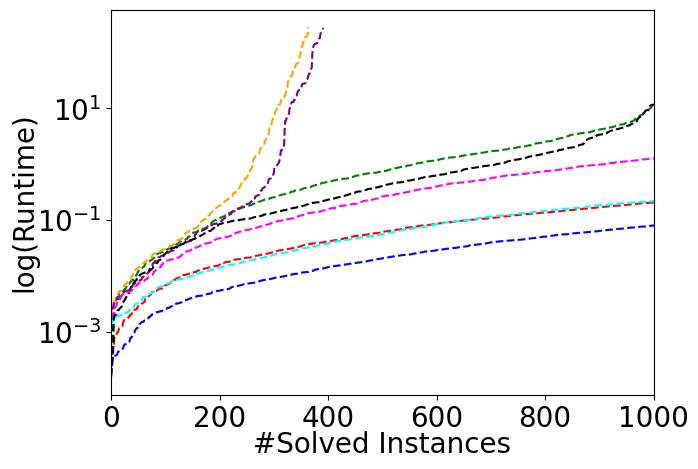
\includegraphics[width=\columnwidth]{Figures/warehouse/mixed_small_figures/Cactus.png}
      % \includegraphics[scale=.2]{Figures/warehouse/mixed_small_figures/DeltaSOC(UEs).png}
      % \caption{Warehouse grids results.}
      % \label{fig:rt-soc-warehouse}
    \end{subfigure}
    \begin{subfigure}[b]{0.69\columnwidth}\centering
      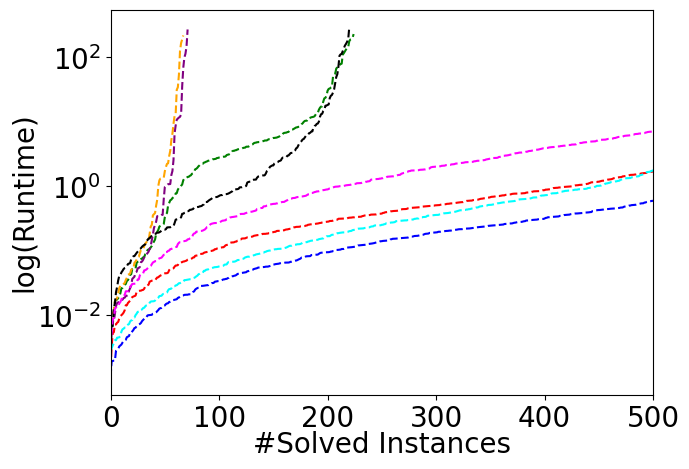
\includegraphics[width=\columnwidth]{Figures/room/mixed_small_figures/Cactus.png}
      % \includegraphics[scale=.2]{Figures/room/mixed_small_figures/DeltaSOC(UEs).png}
      % \caption{Room grids results.}
      % \label{fig:rt-soc-room}
    \end{subfigure}
    \caption{Number of solved problems per runtime for Maze (left), Warehouse (middle), and Rooms (right).}
    \label{fig:rt-soc-results}
\end{figure*}
}

\begin{figure*}[tbhp]
    \begin{subfigure}[b]{0.9\columnwidth}\centering
      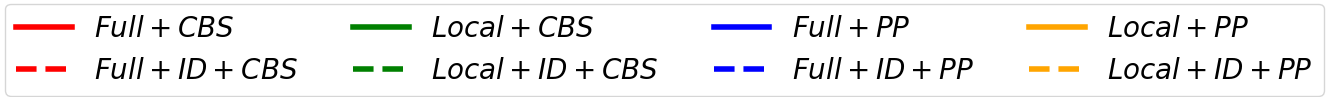
\includegraphics[width=\columnwidth]{Figures/legends_cactus_dashed_lines.png}
      % \caption{Legend}
      % \label{fig:mazelegends}
    \end{subfigure}\\
    \centering
    \begin{subfigure}[b]{0.69\columnwidth}\centering
      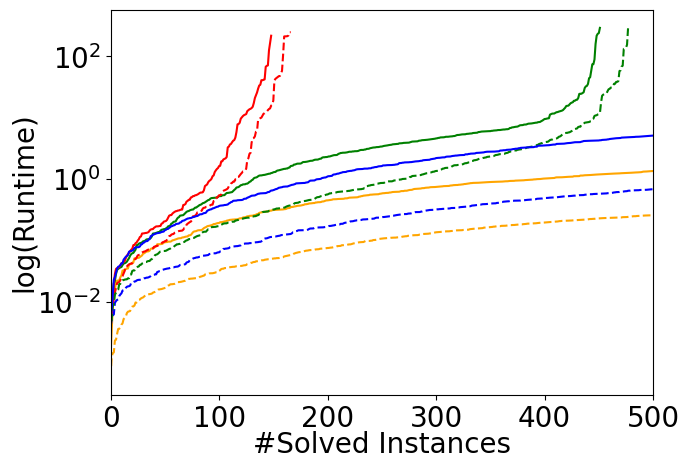
\includegraphics[width=\columnwidth]{Figures/maze/mixed_small_figures/cactus_with_dashed_lines.png}
      % {Figures/maze/mixed_small_figures/Cactus.png}
      % \includegraphics[scale=.2]{Figures/maze/mixed_small_figures/DeltaSOC(UEs).png}
      % \caption{Maze grids results.}
      % \label{fig:rt-soc-maze}
    \end{subfigure}
    \begin{subfigure}[b]{0.69\columnwidth}\centering
      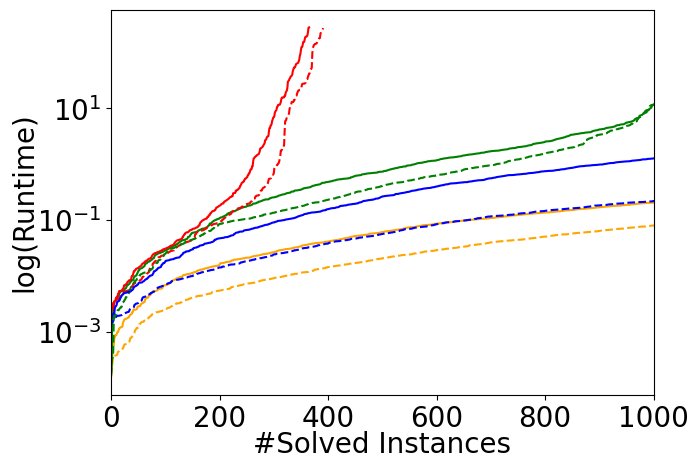
\includegraphics[width=\columnwidth]{Figures/warehouse/mixed_small_figures/cactus_with_dashed_lines.png}
      % \includegraphics[scale=.2]{Figures/warehouse/mixed_small_figures/DeltaSOC(UEs).png}
      % \caption{Warehouse grids results.}
      % \label{fig:rt-soc-warehouse}
    \end{subfigure}
    \begin{subfigure}[b]{0.69\columnwidth}\centering
      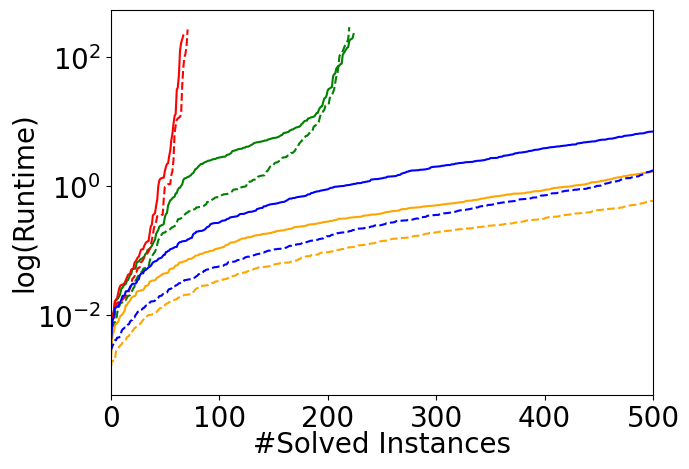
\includegraphics[width=\columnwidth]{Figures/room/mixed_small_figures/cactus_with_dashed_lines.png}
      % \includegraphics[scale=.2]{Figures/room/mixed_small_figures/DeltaSOC(UEs).png}
      % \caption{Room grids results.}
      % \label{fig:rt-soc-room}
    \end{subfigure}
    \caption{Number of solved problems per runtime for Maze (left), Warehouse (middle), and Rooms (right).}
    \label{fig:cactus-w-dashed-lines}
\end{figure*}

In this section, we provide the results of a series of experiments conducted to assess the suggested algorithms across various scenarios. All algorithms were implemented in C++ and our experiments were conducted on a Ubuntu 22.04.2  machines with an Intel Core i7 processor running at a clock speed of 2.8GHz and 16GB RAM.

\subsection{Experimental Setup}
% Grids
We evaluate our algorithms on three diverse grid maps taken from the standard grid MAPF benchmark~\cite{stern2019multi}, namely \texttt{maze-128-128-10} (Maze),
\texttt{room-32-32-4} (Rooms), and
\texttt{warehouse-20-40-10-2-1} (Warehouse),
for problems with up to 130 agents.
% Start and goal locations
To define the agents' start and goal locations in each experiment, we used the 25 \texttt{even} scenarios associated with each grid in the benchmark. These scenario files specify start and goal locations for different numbers of agents such that the resulting MAPF problem is solvable.
% True graph
To define MAPF-IM problems, we created the true graph by adding and removing obstacles from the given grid.
Specifically, for each grid $G$ we created 5 different grids $G_{10}$,
$G_{20}$, $G_{30}$, $G_{40}$, and $G_{50}$, where $G_i$ was created by adding $i$ new obstacles and removing $i$ existing obstacles. In all experiments we assume that $\eko=\emptyset$ initially, while $\ekb$ contains all non-neighbor pairs of positions in the grid. That is, we assume that all edges are uncertain to begin with, except for shortcuts between remote positions that we know do not exist.
The added and removed obstacles were strategically placed to affect the agents' paths to their goals. Figure~\ref{fig:grids} shows grid examples where green and red cells denote the removed and added obstacles, respectively.
In each experiment, we select one of these generated maps to serve as the true graph. We implemented a basic CBS  \cite{sharon2015conflict} with SIPP \cite{phillips2011sipp} as its low-level solver, and also implemented PP with randomized priorities and restarts \cite{bennewitz2001optimizing}.

% Compared algorithms and metrics
In our experiments, we compare all 8 combination of algorithms presented in the paper, i.e., using PP or CBS as the underlying MAPF solver,
with or without ID, and using Full or Local replanning.
In each experiment, we run the evaluated algorithm for with a 5 minute timeout.
The main metrics we consider are (1) runtime until a solution is found;
(2) success rate, i.e., the ratio of problems solved within the 5 minute time limit; and (3) sum of costs (SOC) of the resulting solution.
Preliminary experiments showed that, as expected, the snapshot optimal algorithms (Full+CBS, and Full+ID+CBS) yielded solutions with the lowest SOC. While both yield similar solution quality, they are not identical, due to different tie-breaking, causing the agents to move to places where shortcuts in $\eab$ or blocked edges in $\eao$ result in different path costs.
For the other algorithms, we report the average relative difference between the SOC they obtain and the SOC of Full+CBS, denoted $\Delta SOC$.
% To provide context, we report the difference between the SOC of


\subsection{Results}

% \begin{figure}[tbh]
%     \begin{subfigure}[b]{0.9\columnwidth}\centering
%       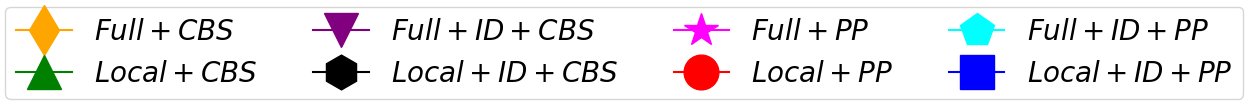
\includegraphics[width=\columnwidth]{Figures/legends -sorted.png}
%       \caption{Legend}
%       \label{fig:mazelegends}
%     \end{subfigure}\\
%     \centering
%     \begin{subfigure}[b]{0.95\columnwidth}\centering
%       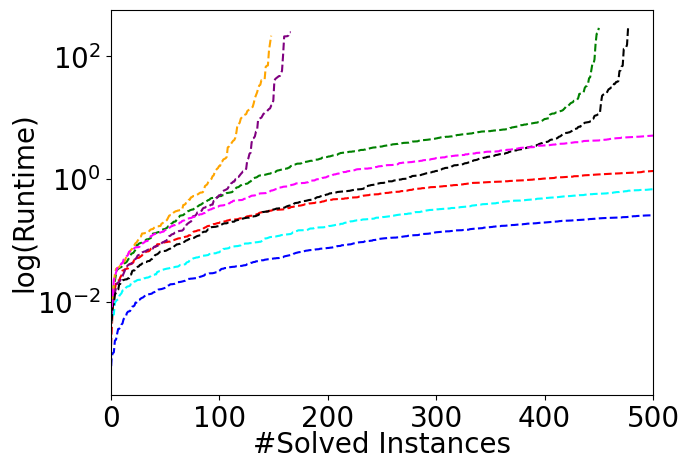
\includegraphics[scale=.2]{Figures/maze/mixed_small_figures/Cactus.png}
%       \includegraphics[scale=.2]{Figures/maze/mixed_small_figures/DeltaSOC(UEs).png}
%       \caption{Runtime and $\Delta$ SOC for Maze grids.}
%       \label{fig:rt-soc-maze}
%     \end{subfigure}
%     \begin{subfigure}[b]{0.95\columnwidth}\centering
%       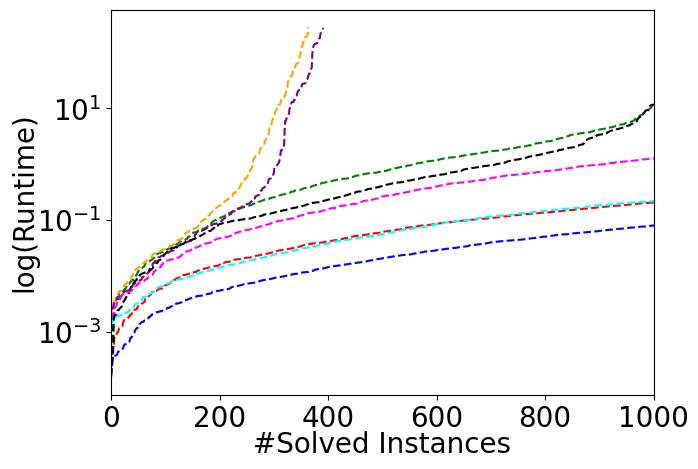
\includegraphics[scale=.2]{Figures/warehouse/mixed_small_figures/Cactus.png}
%       \includegraphics[scale=.2]{Figures/warehouse/mixed_small_figures/DeltaSOC(UEs).png}
%       \caption{Runtime and $\Delta$ SOC for Warehouse grids.}
%       \label{fig:rt-soc-warehouse}
%     \end{subfigure}\\
%     \begin{subfigure}[b]{0.95\columnwidth}\centering
%       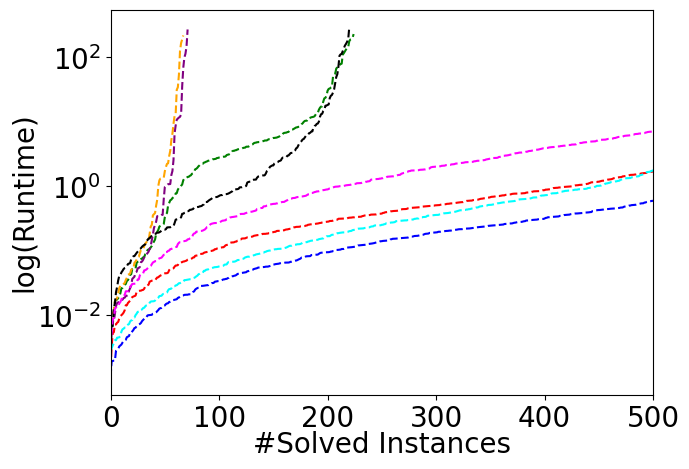
\includegraphics[scale=.2]{Figures/room/mixed_small_figures/Cactus.png}
%       \includegraphics[scale=.2]{Figures/room/mixed_small_figures/DeltaSOC(UEs).png}
%       \caption{Runtime and $\Delta$ SOC for Room grids.}
%       \label{fig:rt-soc-room}
%     \end{subfigure}
%     \caption{Runtime and $\Delta$SOC results.}
%     \label{fig:rt-soc-results}
% \end{figure}

%%%%%%%%%%%%%RETURN ME
% \begin{figure}[tbhp]
%     \begin{subfigure}[b]{0.9\columnwidth}\centering
%       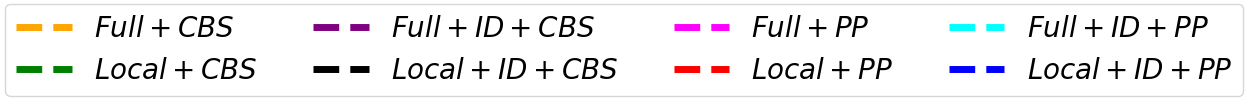
\includegraphics[width=\columnwidth]{Figures/legends-cactus.png}
%       \caption{Legend}
%       \label{fig:mazelegends}
%     \end{subfigure}\\
%     \centering
%     \begin{subfigure}[b]{0.75\columnwidth}\centering
%       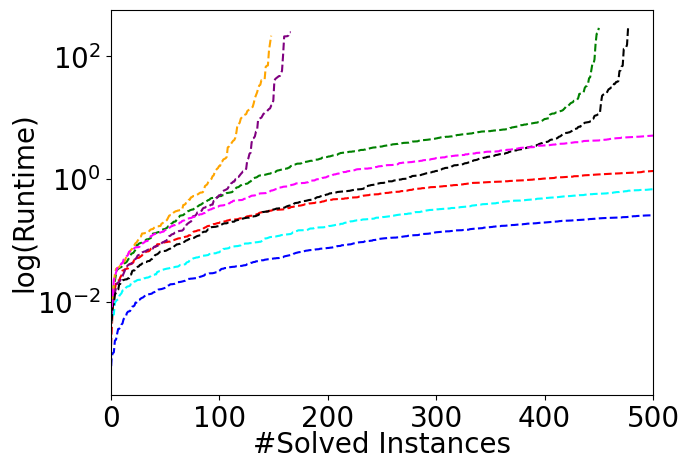
\includegraphics[width=\columnwidth]{Figures/maze/mixed_small_figures/Cactus.png}
%       % \includegraphics[scale=.2]{Figures/maze/mixed_small_figures/DeltaSOC(UEs).png}
%       \caption{Maze grids results.}
%       \label{fig:rt-soc-maze}
%     \end{subfigure}
%     \begin{subfigure}[b]{0.75\columnwidth}\centering
%       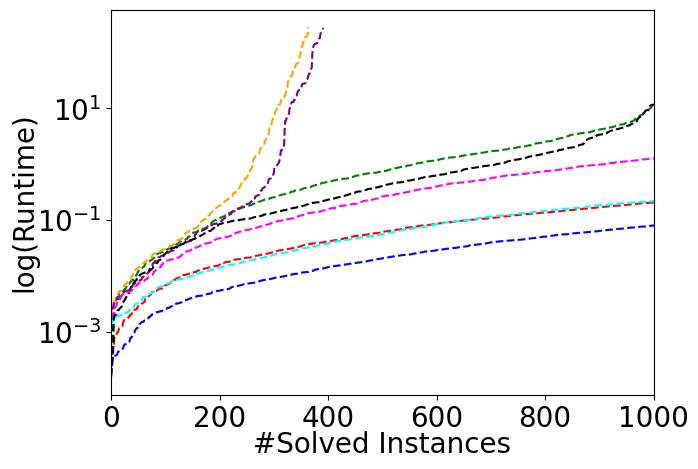
\includegraphics[width=\columnwidth]{Figures/warehouse/mixed_small_figures/Cactus.png}
%       % \includegraphics[scale=.2]{Figures/warehouse/mixed_small_figures/DeltaSOC(UEs).png}
%       \caption{Warehouse grids results.}
%       \label{fig:rt-soc-warehouse}
%     \end{subfigure}\\
%     \begin{subfigure}[b]{0.75\columnwidth}\centering
%       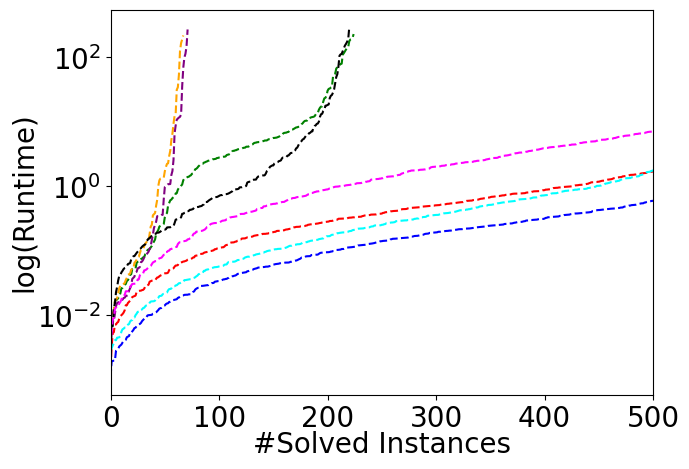
\includegraphics[width=\columnwidth]{Figures/room/mixed_small_figures/Cactus.png}
%       % \includegraphics[scale=.2]{Figures/room/mixed_small_figures/DeltaSOC(UEs).png}
%       \caption{Room grids results.}
%       \label{fig:rt-soc-room}
%     \end{subfigure}
%     \caption{Number of problem solvers per runtime.}
%     \label{fig:rt-soc-results}
% \end{figure}


Figure~\ref{fig:cactus-w-dashed-lines} shows the number of solved problems  ($x$-axis) by each algorithm for a given runtime ($y$-axis).
The results show several trends across all grid types.
First, using ID (dashed) is always beneficial across all configurations, allowing more problems to be solved for the same runtime. Second, as expected, local replanning is significantly faster than full replanning, especially for CBS-based methods.  Finally, again expected, using PP as the underlying CMAPF solver allows solving significantly more problems than using CBS. For example, all PP-based solvers were able to solve over 500 instances within the timeout while all CBS-based algorithms fail to do so.

%%%%%%%%%%%%%RETURN ME
\begin{table}
\centering
\footnotesize
\begin{tabular}{@{}l|cccccc@{}}
% \resizebox{0.95\columnwidth}{!}{
\toprule
% Map/Algo  & Local+CBS & Full+PP & Local+PP & Full+ID+PP & Local+ID+PP \\ \midrule
Map/Algo  & L+C & L+I+C & F+P & L+P & F+I+P & L+I+P \\ \midrule
Maze      & \textbf{0.28\%} & 0.48\%     & 1.84\%    & 1.60\%     & 5.37\%       & 5.74\%       \\
Rooms     & \textbf{0.37\%}  & 0.44\%    & 4.28\%    & 3.96\%     & 4.91\%       & 6.48\%        \\
Warehouse & \textbf{1.66\%}  & 2.24\%    & 3.75\%    & 3.60\%     & 4.49\%       & 4.58\%        \\ \bottomrule
\end{tabular}
% }
    \caption{$\Delta$ SOC, L=local, C=CBS, F=Full, P=PP, and I=ID.}
    \label{tab:delta-soc}
\end{table}

While algorithms that do not aim for optimality clearly scale better, they produce lower quality solutions.
Table~\ref{tab:delta-soc} shows the average $\Delta$SOC for each grid and algorithm. We do not show results for Full+CBS and Full+ID+CBS since these algorithms yield the reference SOC value (i.e., $\Delta$SOC=0).
In all grids Local+CBS yields better (lower) solution cost than the PP-based algorithm, which is expected, as CBS is geared towards finding lowest-cost solutions. Local+ID+CBS is only slightly worse.
Second, in most cases Local+ID+PP yielded the worse solutions (highest $\Delta$SOC). This is reasonable as Local and PP both are designed to tradeoff runtime for quality, and PP with ID ignores newly discovered open edges as well.

% Figure~\ref{fig:rt-soc-results}(right) shows the average $\Delta$SOC as a function of the number of uncertain (either added or removed) edges. Here we do not show results for Full+CBS and Full+ID+CBS since these algorithms yield the reference SOC value (i.e., $\Delta$SOC=0).
% The first trend holds for all grids: Local+CBS yields lower solution cost than the PP-based algorithm, which is reasonable since CBS is geared toward finding lowest-cost solutions.
% Second, in most cases Local+ID+PP yielded the worse solutions (highest $\Delta$SOC). This is reasonable since Local and PP both are designed to tradeoff runtime for quality, and PP with ID ignores newly discovered open edges.



\begin{figure}[tbh]
    \begin{subfigure}[b]{0.9\columnwidth}\centering
      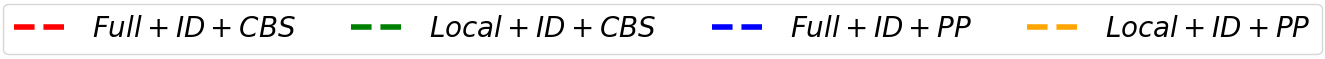
\includegraphics[width=\columnwidth]{Figures/legends_success_rates.png}
      % \caption{Legend}
      % \label{fig:mazelegends}
    \end{subfigure}\\
        \begin{subfigure}[b]{\columnwidth}\centering
      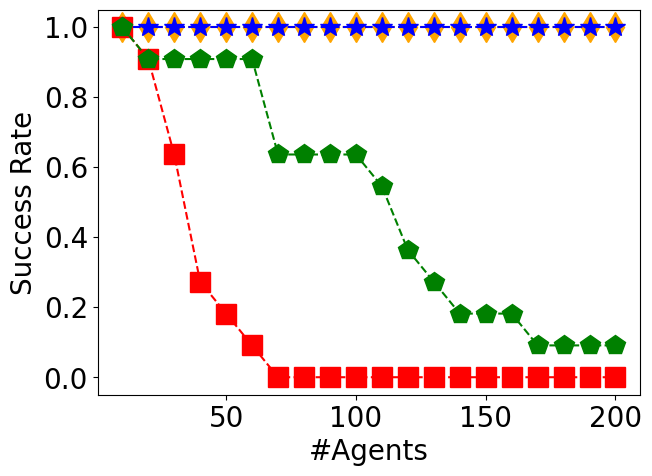
\includegraphics[width=0.47\columnwidth]{Figures/maze/mixed_small_figures/Success-Rate(k)_pos=100_ID_ONLY.png}
      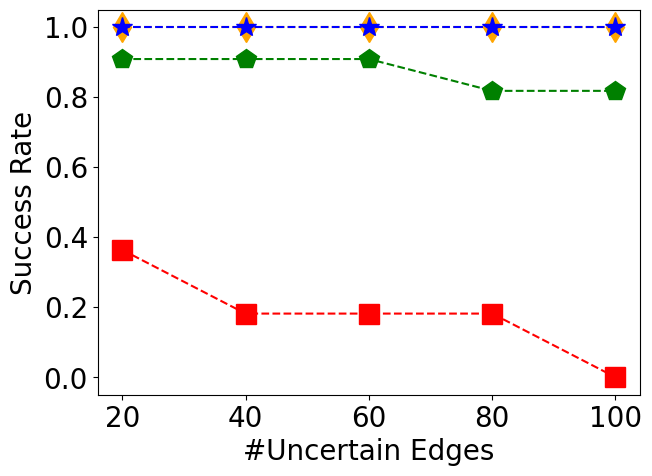
\includegraphics[width=0.47\columnwidth]{Figures/maze/mixed_small_figures/Success-Rate(UEs)_k=50_ID_ONLY.png}
      % \caption{Success-Rate for Maze grids.}
      % \label{fig:mazesrk}
    \end{subfigure}
    \begin{subfigure}[b]{\columnwidth}\centering
      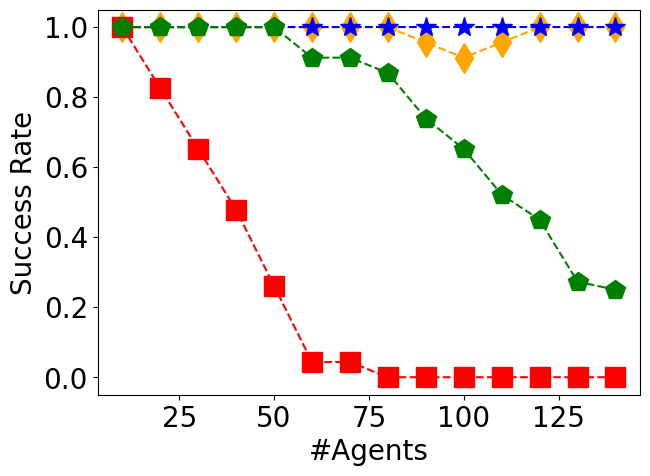
\includegraphics[width=0.47\columnwidth]{Figures/warehouse/mixed_small_figures/Success-Rate(k)_pos=100_ID_ONLY.png}
      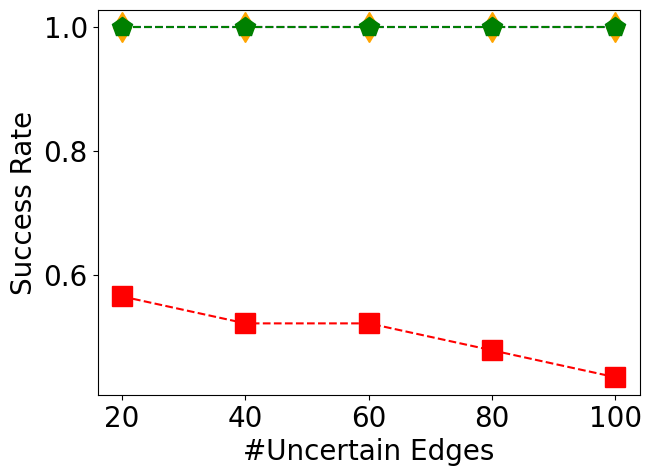
\includegraphics[width=0.47\columnwidth]{Figures/warehouse/mixed_small_figures/Success-Rate(UEs)_k=40_ID_ONLY.png}
      % \caption{Success-Rate for Warehouse grids.}
      % \label{fig:G}
    \end{subfigure}
    \begin{subfigure}[b]{\columnwidth}\centering
      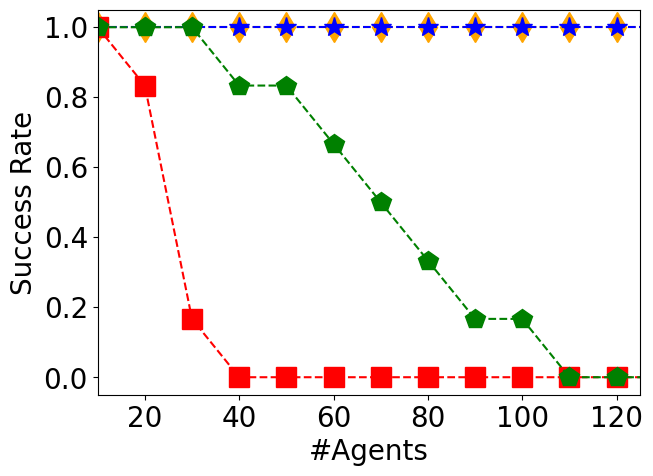
\includegraphics[width=0.47\columnwidth]{Figures/room/mixed_small_figures/Success-Rate(k)_pos=100_ID_ONLY.png}
      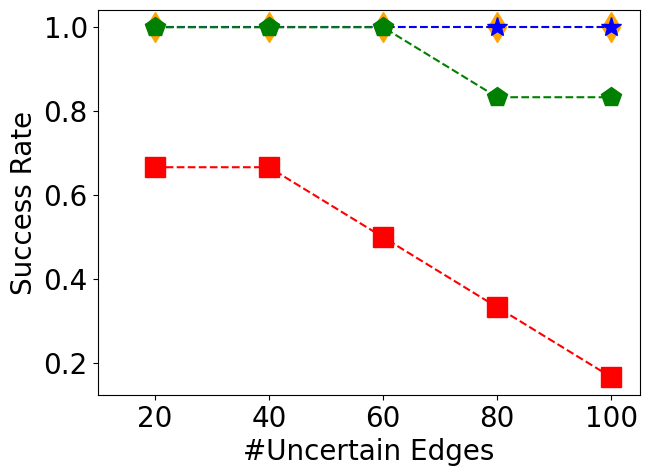
\includegraphics[width=0.47\columnwidth]{Figures/room/mixed_small_figures/Success-Rate(UEs)_k=30_ID_ONLY.png}
      % \caption{Success-Rate for Room grids.}
      % \label{fig:Gs0}
    \end{subfigure}
    \caption{Success rate results for Maze (top), Warehouse (middle), and Rooms (bottom).}
    \label{fig:success-rate}
\end{figure}

\commentout{
\begin{figure}[tbh]
    \begin{subfigure}[b]{0.9\columnwidth}\centering
      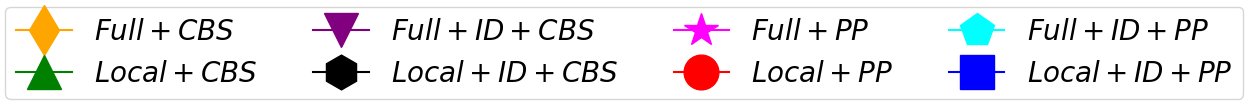
\includegraphics[width=\columnwidth]{Figures/legends -sorted.png}
      % \caption{Legend}
      % \label{fig:mazelegends}
    \end{subfigure}\\
        \begin{subfigure}[b]{\columnwidth}\centering
      \includegraphics[width=0.47\columnwidth]{Figures/maze/mixed_small_figures/Success-Rate(k)_pos=100.png}
      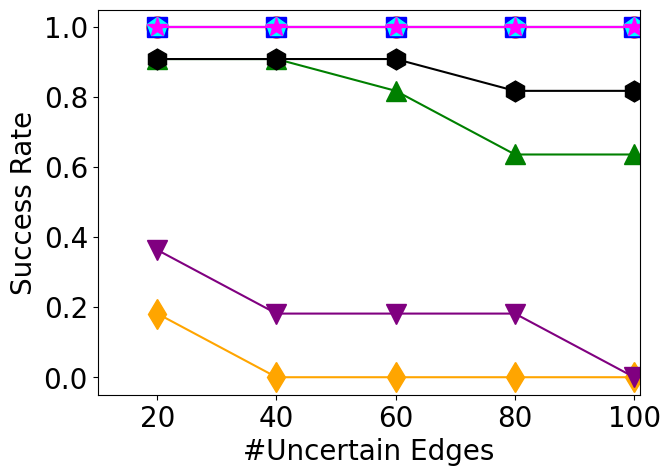
\includegraphics[width=0.47\columnwidth]{Figures/maze/mixed_small_figures/Success-Rate(UEs)_k=50.png}
      % \caption{Success-Rate for Maze grids.}
      % \label{fig:mazesrk}
    \end{subfigure}
    \begin{subfigure}[b]{\columnwidth}\centering
      \includegraphics[width=0.47\columnwidth]{Figures/warehouse/mixed_small_figures/Success-Rate(k)_pos=100.png}
      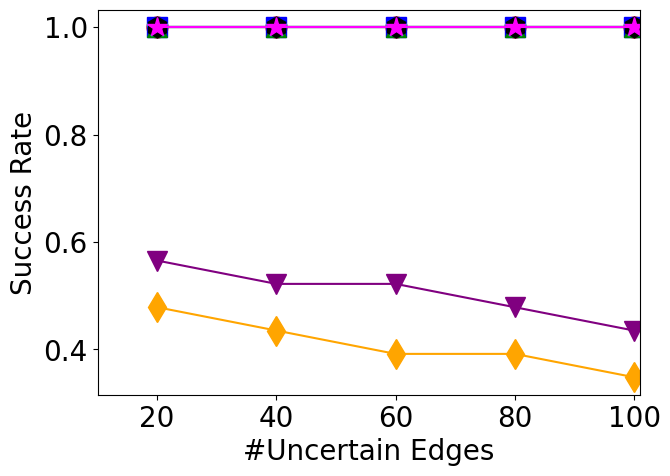
\includegraphics[width=0.47\columnwidth]{Figures/warehouse/mixed_small_figures/Success-Rate(UEs)_k=40.png}
      % \caption{Success-Rate for Warehouse grids.}
      % \label{fig:G}
    \end{subfigure}
    \begin{subfigure}[b]{\columnwidth}\centering
      \includegraphics[width=0.47\columnwidth]{Figures/room/mixed_small_figures/Success-Rate(k)_pos=100.png}
      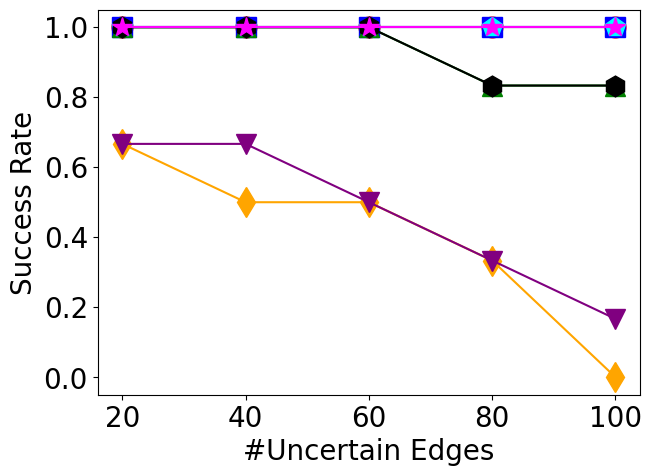
\includegraphics[width=0.47\columnwidth]{Figures/room/mixed_small_figures/Success-Rate(UEs)_k=30.png}
      % \caption{Success-Rate for Room grids.}
      % \label{fig:Gs0}
    \end{subfigure}
    \caption{Success rate results for Maze (top), Warehouse (middle), and Rooms (bottom). \guy{would be better to have solid-dashed with the same color for with and without ID}}
    \label{fig:success-rate}
\end{figure}
}

% Next, we explore the impact of the problem parameters, namely number of agents and number of uncertain edges, on the algorithms performance.
Figure~\ref{fig:success-rate}(left) plots the success rate ($y$-axis) of each algorithm for an increasing number of agents ($x$-axis), where the number of uncertain edges was fixed and set to 100. As the effect of ID is clear from Figure~\ref{fig:cactus-w-dashed-lines}, we report only the variants with ID.
The same trends observed above are evident: Local replanning, and using PP  significantly reduce the algorithms' runtime and hence increase the success rate.  The same trends are also observed in Figure~\ref{fig:success-rate}(right), where success rate is plotted against varying number of uncertain edges.

From a practical point of view these results suggest that, at least for the particular scenarios that we experimented with, the local version scales much better, and PP scales orders of magnitude better, at a minimal solution quality reduction. The most scalable method: Local+ID+PP suffers at most $6.5\%$ quality reduction. That is, if it is important to scale to larger problems, it is a very practical approach.

% Figure ~\ref{fig:mazesrues} plots the success rate ($y$-axis) of each algorithm for an increasing number of uncertain edges ($x$-axis), where the number of agents was fixed and set to 50.


% \plan{Results mixed}

% First, consider the results for Maze maps, given in figure~\ref{fig:maze_mixed_all}.
% \plan{SuccessRate(k)}

% % Figure Y (Z) plots the number of problems solved ($x$-axis) by each algorithm  for a given runtime ($y$-axis).
% % The results show several trends.
% % First, .... the trend ... for example ...numeric example.

% \commentout{
%     local > full
%     id > ra
%     local+CBS return nearly snapshot-optimal policies
%     runtime: id+pp > pp > local+cbs > ra + cbs
% }

% Figure ~\ref{fig:mazesrk} plots the success rate ($y$-axis) of each algorithm for an increasing number of agents ($x$-axis), where the number of uncertain edges was fixed and set to 100. The results clearly demonstrates that policy adaption with id technique indeed aids in either CBS or PP based frameworks. For example, given 40 agents scenarios, ID outperformed AlwaysReplan approach by approximately ten percent.

% Figure ~\ref{fig:mazesrues} plots the success rate ($y$-axis) of each algorithm for an increasing number of uncertain edges ($x$-axis), where the number of agents was fixed and set to 50.



% \plan{SOC}
% \plan{Impact of number of changed edges}
% \plan{Impact of number of agents}


% % NOT NOW

% \plan{Results only open}


% \plan{Results mixed}



% \begin{figure*}[tbh]
%     \begin{subfigure}[b]{\textwidth}\centering
%       \includegraphics[scale=.3]{Figures/legends.png}
%       \caption{Legend}
%       \label{fig:Gs1}
%     \end{subfigure}

%         \centering
%     \begin{subfigure}[b]{0.45\columnwidth}\centering
%       \includegraphics[scale=0.2]{Figures/maze/mixed/Success-Rate(k)_pos=100.png}
%       \caption{Maze}
%       \label{fig:G}
%     \end{subfigure}
%     \begin{subfigure}[b]{0.45\columnwidth}\centering
%       \includegraphics[scale=.2]{Figures/maze/mixed/Success-Rate(k)_pos=100.png}
%       \caption{Rooms}
%       \label{fig:Gs0}
%     \end{subfigure}
%     \begin{subfigure}[b]{0.45\columnwidth}\centering
%       \includegraphics[scale=.2]{Figures/maze/mixed/Success-Rate(k)_pos=100.png}
%       \caption{Random}
%       \label{fig:PlanGs0}
%     \end{subfigure}
%     \begin{subfigure}[b]{0.45\columnwidth}\centering
%       \includegraphics[scale=.2]{Figures/maze/mixed/Success-Rate(k)_pos=100.png}
%       \caption{Warehouse}
%       \label{fig:Gs1}
%     \end{subfigure}

%     \caption{Example to illustrate needed size.}
%     \label{fig:ProbelmDefinition}
% \end{figure*}

% \begin{figure*}[tbh]
%     \begin{subfigure}[b]{\textwidth}\centering
%       \includegraphics[scale=.3]{Figures/legends -sorted.png}
%       \caption{Legend}
%       \label{fig:mazelegends}
%     \end{subfigure}

%         \centering
%     \begin{subfigure}[b]{0.45\columnwidth}\centering
%       \includegraphics[scale=0.2]{Figures/maze/mixed_small_figures/Success-Rate(k)_pos=100.png}
%       \caption{Success-Rate(k)}
%       \label{fig:mazesrk}
%     \end{subfigure}
%     \begin{subfigure}[b]{0.45\columnwidth}\centering
%       \includegraphics[scale=.2]{Figures/maze/mixed_small_figures/Success-Rate(UEs)_k=50.png}
%       \caption{Success-Rate(UEs)}
%       \label{fig:mazesrues}
%     \end{subfigure}
%     \begin{subfigure}[b]{0.45\columnwidth}\centering
%       \includegraphics[scale=.2]{Figures/maze/mixed_small_figures/Cactus.png}
%       \caption{Runtime}
%       \label{fig:mazert}
%     \end{subfigure}
%     \begin{subfigure}[b]{0.45\columnwidth}\centering
%       \includegraphics[scale=.2]{Figures/maze/mixed_small_figures/DeltaSOC(UEs).png}
%       \caption{DeltaSOC(UES)}
%       \label{fig:mazedsoc}
%     \end{subfigure}

%     \caption{maze-128-128-10}
%     \label{fig:maze_mixed_all}
% \end{figure*}






% \begin{figure*}[tbh]
%     \begin{subfigure}[b]{\textwidth}\centering
%       \includegraphics[scale=.3]{Figures/legends -sorted.png}
%       \caption{Legend}
%       \label{fig:Gs1}
%     \end{subfigure}
%     \begin{subfigure}[b]{0.45\columnwidth}\centering
%       \includegraphics[scale=0.2]{Figures/warehouse/mixed_small_figures/Success-Rate(k)_pos=100.png}
%       \caption{Success-Rate(k)}
%       \label{fig:G}
%     \end{subfigure}
%     \begin{subfigure}[b]{0.45\columnwidth}\centering
%       \includegraphics[scale=.2]{Figures/warehouse/mixed_small_figures/Success-Rate(UEs)_k=40.png}
%       \caption{Success-Rate(UEs)}
%       \label{fig:Gs0}
%     \end{subfigure}
%     \begin{subfigure}[b]{0.45\columnwidth}\centering
%       \includegraphics[scale=.2]{Figures/warehouse/mixed_small_figures/Cactus.png}
%       \caption{Runtime}
%       \label{fig:PlanGs0}
%     \end{subfigure}
%     \begin{subfigure}[b]{0.45\columnwidth}\centering
%       \includegraphics[scale=.2]{Figures/warehouse/mixed_small_figures/DeltaSOC(UEs).png}
%       \caption{$\Delta$ SOC(UES)}
%       \label{fig:Gs1}
%     \end{subfigure}

%     \caption{warehouse-20-40-10-2-1}
%     \label{fig:warehouse_mixed_all}
% \end{figure*}





% \begin{figure*}[tbh]
%     \begin{subfigure}[b]{\textwidth}\centering
%       \includegraphics[scale=.3]{Figures/legends -sorted.png}
%       \caption{Legend}
%       \label{fig:Gs1}
%     \end{subfigure}

%         \centering
%     \begin{subfigure}[b]{0.45\columnwidth}\centering
%       \includegraphics[scale=0.2]{Figures/room/mixed_small_figures/Success-Rate(k)_pos=100.png}
%       \caption{Success-Rate(k)}
%       \label{fig:G}
%     \end{subfigure}
%     \begin{subfigure}[b]{0.45\columnwidth}\centering
%       \includegraphics[scale=.2]{Figures/room/mixed_small_figures/Success-Rate(UEs)_k=30.png}
%       \caption{Success-Rate(UEs)}
%       \label{fig:Gs0}
%     \end{subfigure}
%     \begin{subfigure}[b]{0.45\columnwidth}\centering
%       \includegraphics[scale=.2]{Figures/room/mixed_small_figures/Cactus.png}
%       \caption{Runtime}
%       \label{fig:PlanGs0}
%     \end{subfigure}
%     \begin{subfigure}[b]{0.45\columnwidth}\centering
%       \includegraphics[scale=.2]{Figures/room/mixed_small_figures/DeltaSOC(UEs).png}
%       \caption{$\Delta$ SOC(UES)}
%       \label{fig:Gs1}
%     \end{subfigure}

%     \caption{room-64-64-8}
%     \label{fig:room_mixed_all}
% \end{figure*}



\section{Related Work}

%\plan{In related work we need to emphasize novelty - describe a method and then say how we are different}
%1) Tomer Shahar, Shashank Shekhar, Dor Atzmon, Abdallah Saffidine, Brendan Juba, Roni Stern:
%Safe Multi-Agent Pathfinding with Time Uncertainty. J. Artif. Intell. Res. 70: 923-954 (2021)
%They studied the Multi-Agent Pathfinding with Time Uncertainty (MAPF-TU) problem, where we only have %lower and upper bounds on the time it takes to traverse each edge. This is different from our case, %where obstacles may appear.

MAPF under different forms of uncertainty have been studied before.
For example, in MAPF-TU~\cite{shahar2021safe} all edges are known but there are lower and upper bounds on the time it takes to traverse each edge, while in MAPF-DP agents' actions may be delayed with some probability~\cite{honig2016multi, wagner2017path, atzmon2020probabilistic}.
In Online MAPF~\cite{vsvancara2019online} new agents appear over time, while
Queffelec et al.~\shortcite{queffelec2021planning,queffelec2023complexity}
discuss MAPF in partially known environments.
These papers tackle different uncertainty than we do. %, and avoid using plan trees.
Closest to our MAPF-IM problem is recent work on MAPF-OU \cite{shofer2023multi}, where a relatively small subset of edges may be blocked.
%They assume a-priori knowledge of a relatively small set of possibly blocked edges.
MAPF-IM extends this problem setting in two ways. First, we allow both for edges that are considered open, but may be blocked, and for edges that are considered blocked, but may be open. Second, we assume that the set of uncertain edges is very large, and thus, that computing complete plan trees is intractable.


% \cite{vsvancara2019online} study a MAPF variant where new agents might appear over time. They use ID to reuse paths from previous planning iterations. Some of our policy adaption techniques also utilized ID technique, inferring a partitioning of the agent based on previous computations.

% \citet{queffelec2021planning,queffelec2023complexity}  discuss MAPF in partially known environments. They focus on complexity analysis, given constraints such as disallowing collisions, communication, and finite horizon.

% They suggest two offline algorithms that construct plan trees for all agents, branching on the possibly blocked edges. Given the relatively small set of possibly blocked edges, these plan trees can have manageable size.




%Furthermore, in MAPF-TU the time bounds are known a priori, thus offline planning is plausible, while in our setting the problem solver is not aware to uncertain edges, hence planning is deferred.

% In stochastic MAPF \cite{levy2022online}, an agent may stochastically move in a different direction than intended. Aside from the difference in uncertainty, stochastic problems can be optimized for minimizing expected costs, which does not hold for the non-stochastic case.


%(NOT BY ME BUT RELATED)
%2) 	Hang Ma, Jiaoyang Li, T. K. Satish Kumar, Sven Koenig: Lifelong Multi-Agent Path Finding for %Online Pickup and Delivery Tasks. AAMAS 2017: 837-845
%They studied a different online variant of MAPF called lifelong MAPF (LMAPF), where the set of %agents is fixed but an agent reaching its goal will receive a new goal to go to.

% \plan{Bar's work MAPF-OU}



%3) Our work with Bar.
%There they focused offline planning, and require knowledge of all possible obstacle locations. We %plan online, and do not require any a-priori knowledge of where obstacles may appear.


% \plan{Work of Roni}

%\plan{snapshot optimality}
%3) Jirí Svancara, Marek Vlk, Roni Stern, Dor Atzmon, Roman Barták: Online Multi-Agent Pathfinding. %AAAI 2019: 7732-7739
%They studied the online variant of MAPF, where agents appear and disappear over time. In our cases %the set of agents is fixed, but obstacles may appear or disappear.


% \plan{Candian TSP - multi agent version}

% Our problem can also be considered as an extension of the multi-agent Canadian travelers problem (CTP) \cite{zhang2013k}. While there is much work on CTP, only a few papers focus on multi-agent CTP. For example, in the multi-agent O–D $k$-Canadian Traveler Problem \cite{shiri2017online,shiri2019randomized}, there are at most $k$ blocked edges. All the agents start at initial vertex $O$. The objective is to find a pathway for at least one agent to vertex $D$ with minimal cost.  They also use an online strategy, given the size of the complete solution. We extend these settings in several ways: first, we assume both possibly blocked and possibly open edges, second, we do not assume a joint origin and destination for all agents, and third, we allow for a more flexible observation model, allowing sensing edges not only from their immediate vertices. Finally, they attempt to find a policy that with high probability minimizes cost, focusing on the exploration strategy, while we attempt to provably minimize costs when the assumptions over the edges are accurate. Also, research in CTP does not consider the problem of collisions, which pose a major challenge for us.

Our problem is somewhat related to the Canadian Travelers Problem (CTP) \cite{zhang2013k}, which is a pathfinding problem in which some edges may be blocked. While there is much work on CTP, only a few papers focus on multi-agent CTP~\cite{shiri2017online,shiri2019randomized}.
MAPF-IM is different from (multi-agent) CTP in several ways. First, in MAPF-IM edges may become either blocked or open. Second, in CTP all agents start in the same location while in MAPF-IM each agent has its own start.
% Third, our sensing action is more flexible, allowing sensing edges not only from their immediate vertices. [[Roni: risky]]
Finally, in CTP collisions are not considered while in MAPF-IM they are key constraints.
%they attempt to find a policy that with high probability minimizes cost, focusing on the exploration strategy, while we attempt to provably minimize costs when the assumptions over the edges are accurate. Also, research in CTP does not consider the problem of collisions, which pose a major challenge for us.
% For example, in the multi-agent O–D $k$-Canadian Traveler Problem \cite{shiri2017online,shiri2019randomized}, there are at most $k$ blocked edges. All the agents start at initial vertex $O$. The objective is to find a pathway for at least one agent to vertex $D$ with minimal cost.  They also use an online strategy, given the size of the complete solution. We extend these settings in several ways: first, we assume both possibly blocked and possibly open edges, second, we do not assume a joint origin and destination for all agents, and third, we allow for a more flexible observation model, allowing sensing edges not only from their immediate vertices. Finally, they attempt to find a policy that with high probability minimizes cost, focusing on the exploration strategy, while we attempt to provably minimize costs when the assumptions over the edges are accurate. Also, research in CTP does not consider the problem of collisions, which pose a major challenge for us.
Multi-Robot SLAM (MR-SLAM)~\cite{burgard2000collaborative,kshirsagar2018survey,abdulgalil2019multi}, is also somewhat similar to MAPF-IM. SLAM typically assumes a mostly unknown environment and the objective is to map the environment, while we focus on a mostly known environment and the objective is to navigate the agents towards their goals.
%They also typically limit their attention to physical environments and sensors, while we study a more abstract problem setting. \roni{Last sentence should be commented out in my opinion as it is not clear. }
% MR-SLAM research mostly focuses on synchronizing the information collected from the noisy sensors of agents into a single map. Subsequently they assume that navigation is less important. Our work can hence be considered as complementing work on MR-SLAM, assuming perfect sensors and simple map synchronization, and focusing instead on the navigation problem.


% The setting and objective in MR-SLAM is typically different: they assume a mostly unknown environment and the objective is to map the environment, while we focus on a mostly known environment and the objective is to navigate the agents towards their goals.
% %They also typically limit their attention to physical environments and sensors, while we study a more abstract problem setting. \roni{Last sentence should be commented out in my opinion as it is not clear. }
% MR-SLAM research mostly focuses on synchronizing the information collected from the noisy sensors of agents into a single map. Subsequently they assume that navigation is less important. Our work can hence be considered as complementing work on MR-SLAM, assuming perfect sensors and simple map synchronization, and focusing instead on the navigation problem.

We propose a specific approach for reusing information collected in previous replanning episodes by intelligently selecting which agents should replan. Orthogonality, one may use incremental search methods such as $D^*$-lite~\cite{koenig2002d} and $LPA^*$~\cite{koenig2004lifelong} for the individual planning~\cite{boyarski2021iterative}. We leave integration of these ideas to future research.





\section{Conclusion and Future Work}

This paper examines a novel form of MAPF known as MAPF-IM, in which the problem solver has limited knowledge about the traversability of certain edges. We formally defined the MAPF-IM problem and proposed several frameworks for addressing it: one generates a collision-free policy once the ongoing policy need to be revised, whereas the second defer conflict resolution until it occurs within at most $r$ timesteps. Furthermore, we suggested two incremental methods for policy adaption, which applies ID technique over either CBS or PP. In our experimental study, we demonstrate the scalability of our approaches in various domains with respect to the number of agents and the amount of unknown edges. Our study paves the way for other research inquiries, such as addressing the challenges of solving MAPF-IM in settings characterised by communication delays or high costs, exploration-eploitation tradeoffs, and more.

\clearpage
\bibliography{aaai24}
\end{document}


% \begin{algorithm}[t]
% \caption{ID (BAD NAME)}
%     \label{alg:ID}
% \footnotesize
% \SetKwBlock{Main}{Main}{end}
% \SetKwInOut{Input}{Input:}
% \SetKwInOut{Output}{Output:}
% \Input{graph $G=\langle V, E, \eo, \eb \rangle$, snapshot $G_s=\langle V, \eko, \ekb, \eao, \eab \rangle$, observation relation $O$, set of agents $A$}
%     $\pi \leftarrow PlanCMAPF(G', A)$\\
%     \While{not all agents reached their goals}{
%         Execute next step according to $\pi$, obtain new snapshot $G'_s$\\
%         % If map inaccuracy detected
%         \If{$E'_{ko} \neq E_{ko} \vee E'_{kb} \neq E_{kb}$}{
%             Update $G'_s$ with new knowledge\\
%             Affected$\gets$ detected affected agents
%             Replan for all the agents in Affected\\
%             Update $\pi$
%             break
%         }
%     }
%     \Return{$\pi$}
% \end{algorithm}

% \begin{algorithm}[t]
% \caption{DetectedAffected}
%     \label{alg:affected}
% \footnotesize
% \SetKwBlock{Main}{Main}{end}
% \SetKwInOut{Input}{Input:}
% \SetKwInOut{Output}{Output:}
% \Input{graph $G=\langle V, E, \eo, \eb \rangle$, snapshot $G_s=\langle V, \eko, \ekb, \eao, \eab \rangle$,
% If new open edge: all are affected
% Else
%     If PP, highest priority agent that planned to path in the blocked cell and all lower priority agents
%     If CBS, ... the stuff with the groups  ...
% \end{algorithm}



% \subsection{Roni Suggested Design}

% \begin{algorithm}[t]
% \caption{Full plan framework}
%     \label{alg:execution}
% \footnotesize
% \SetKwBlock{Main}{Main}{end}
% \SetKwInOut{Input}{Input:}
% \SetKwInOut{Output}{Output:}
%     $\pi$ create initial plan based on snapshot \\
%     \While{not all agents reached their goals}{
%         If change in snapshot -- call \textbf{AdaptPlan(all agents, change description)} to update $\pi$ \\
%         Execute next step in $\pi$ \\
%     }
% \end{algorithm}

% \begin{algorithm}[t]
% \caption{AdaptPlan --- adapt a given plan based on detected change in the snapshot}
%     \label{alg:adapt-plan}
% \footnotesize
% \SetKwBlock{Main}{Main}{end}
% \SetKwInOut{Input}{Input: agents, new snapshot, change location, type of change}
% \SetKwInOut{Output}{Output: new plan for agents}
%     Option 1: replan all according to new snapshot
%     Option 2: replan only for affected agents
%     Option 2.1.: how to detect affected in CBS
%     Option 2.2.: how to detect affected in PP
% \end{algorithm}


% \begin{algorithm}[t]
% \caption{Online local plan framework}
%     \label{alg:execution}
% \footnotesize
% \SetKwBlock{Main}{Main}{end}
% \SetKwInOut{Input}{Input:}
% \SetKwInOut{Output}{Output:}
%     $\pi$ create an initial plan based on snapshot \\
%     \While{not all agents reached their goals}{
%         partition $\gets$ split agents based on proximity \\
%         For each partition
%             If conflict within the partition - replan(partition)
%             If change in snapshot -- call \textbf{AdaptPlan(partition change description)} to update $\pi$ \\
%         Execute next step in $\pi$ \\
%     }
% \end{algorithm}

% Experiments:

% Full plan framework:
% Replan All (RA) with PP
% Replan All (RA) with CBS
% IdentifyAffected (IA) with PP
% IdentifyAffected (IA) with CBS

% Local plan framework:
% Replan All with PP
% Replan All with CBS
% IdentifyAffected (IA) with PP
% IdentifyAffected (IA) with CBS


% Expected trends:

% 1. Major comparison: who is faster: Full+RA+PP vs. Local+RA+PP vs. Local+IA+PP
% Expected: Online+IA+PP will be the fastest, maybe by a marginal amount. Look at the harders instances.

% 2. Major comparison #2: who is faster among snapshot optimal: Full+RA+CBS vs.  Full+IA+CBS
% Expected: Full+IA+CBS is much faster

% 3. Other comparisons #1: is there a benefit in snapshopt optimal in terms of SOC: all solvers
% Expected: (a) CBS-based better than PP (b) Full finds better local, (c) IA and RA are the same
% Also expected: Full and Local are practically the same.

% 4. Other comparison #2: impact of number of changes (x-axis is the number of changes, y-performance (success rate or runtime) )
% Expected: as there are more differences between the initial snapshot and the real graph,
% there advantage of IA over RA will increase.

% 5. Other comparison #3: impact of type of changes (only open, only closed, ideally: graph with middle grounds)
% Expected: as we have more closed obstacles, we expected better advantage of IA over RA

% for only closed, only blocked, mixed:
%     1 + 2: CACTUS
%     3: AverageSOC(K), AVERAGESOC(UE)
%     4. SuccessRate(K), SuccessRate(UEs)



% \subsection{End of Roni Suggested Design}